\documentclass[conference]{IEEEtran}
\IEEEoverridecommandlockouts
% The preceding line is only needed to identify funding in the first footnote. If that is unneeded, please comment it out.
\usepackage{cite}
\usepackage[hidelinks]{hyperref}
\usepackage{amsmath,amssymb,amsfonts}
\usepackage{algorithm}
\usepackage{algorithmic}
\usepackage{graphicx}
\usepackage{textcomp}
\usepackage{xcolor}
\usepackage{booktabs}
\usepackage{placeins}


\def\BibTeX{{\rm B\kern-.05em{\sc i\kern-.025em b}\kern-.08em
    T\kern-.1667em\lower.7ex\hbox{E}\kern-.125emX}}

\newtheorem{example}{Example}
\newtheorem{theorem}{Theorem}
\newcommand{\model}{\mathcal{M}}
\newcommand{\qfunc}{\mathcal{Q}}
\newcommand{\qfunctarget}{\mathcal{Q'}}
\newcommand{\Mstate}{\mathbf{s}}
\newcommand{\Maction}{\mathbf{a}}
\newcommand{\Mnextstate}{\mathbf{s'}}
\newcommand{\reals}{\mathbb{R}}

\DeclareMathOperator*{\argmax}{arg\,max}
\DeclareMathOperator*{\argmin}{arg\,min}

\begin{document}

\title{CS556 Project 1 - Modeling Worm Propagation in Large Networks\\
}

\author{\IEEEauthorblockN{Alperen Tercan}
\IEEEauthorblockA{\textit{Department of Computer Science} \\
\textit{Colorado State University}\\
Fort Collins, US \\
alperen.tercan@colostate.edu}
}

\maketitle

% \begin{abstract}
% \end{abstract}

% \begin{IEEEkeywords}
% component, formatting, style, styling, insert
% \end{IEEEkeywords}

\section{Introduction}

In this report, we will investigate how an internet worms spread under topology constraints. This analysis can be considered as a generalized version of \cite{redcode}, which models and analysis propagation of Code Red worm without topology constraints. No topology constraint is equivalent to a fully connected graph.

\section{Methods}

In this section, our experimental setup will be described.

\subsection{Simulation}

To simulate the spread of infection, we run a discrete-time simulation where each round infected nodes try to infect their susceptible neighbors according to a spread model that will be discussed in \autoref{sec:spread_model}. The simulation continues until there isn't any node left that can be infected.

When the cure is introduced, we extended our approach to a turn-based simulation. Each round consist of two phases: infection and cure. During the infection phase, infection spreads to uncured and uninfected nodes. Then, in the cure phase, cure spreads according to the same spread model. The simulation continues until there aren't any infected nodes left.


\subsection{Spread Model}\label{sec:spread_model}

When modeling the spread of the infection, we have considered three different approaches. Firstly, we considered an unlimited resource scenario where an infected node can infect unlimited number of adjacent susceptible nodes at each simulation step. Following RedCode example, this would be assuming the number of threads an infected computer can run in parallel is infinite. However, since the networks that we use are topology constrained; number of threads is still limited by the degree of the node. In this model, every round, each infected node samples $d$ random values from a Bernoulli distribution with $p = p_{\text{inf}}$, where d is the degree of the node and $p_{\text{inf}}$ is the infection probability. Each value decide whether the corresponding neighbor will be infected or not. We implement this model from the susceptible node point-of-view. So, for each susceptible node, number of infected neighbors, $k$, is computed. Then we sample a random Bernoulli random variable with $p = 1 - (1-p_{\text{inf}})^k$. This approach reduces number of random variables to sample.

A second approach was to limit the number susceptible neighbors an infected node can try to infect every round by a hyperparameter $m$. For example, in RedCode example, $m$ was $~100$, the number of threads. It is important to note that for scale-free graphs, degree of some hub nodes can be very large; hence, making a realistic choice of $m$ important. Whereas, maximum degree of a node in binomial and small-worlds graphs usually small enough to make unlimited case realistic enough, ie. no node will be overwhelmed by the number of susceptible neighbors it has. In this model, every round, $m$ susceptible neighbors are chosen for each infected node. Then, $m$ Bernoulli random variables with $p = p_{\text{inf}}$ are sampled for each infected node to decide whether these neighbors will be infected or not.

A third approach was proposed by Prof. Ray. This limits the number of an infected node can infect instead of try to infect. While the difference may seem subtle, its practical impacts are important. For example, when $m=1$, probability of an infection between an infected node and its susceptible neighbor is $\frac{1}{d}(1-(1-p)^d)$ in the third approach whereas it is $\frac{p}{d}$ in the second; where $d$ is the number of susceptible neighbors of the infected node.

In this report, we will use mainly approach 1 and call it unlimited resources model. If not stated otherwise, assume that this model is used.

We will also do some experiments with the third approach, and we will call it single infection model. While the second approach is also interesting; we won't be presenting any results with it due to space and time constraints.

\subsection{Graph Topologies}

In this work, we experiment with three random graph topologies: binomial, scale-free, and small-worlds. An important decision is
to decide how to define comparable graphs with these different topologies. As each topology is connectivity-wise inherently different; which is also the fact that we're investigating; how to make a fair comparison.

For this, we will compare different topologies consisting of same number nodes, $n$, and edges, $m$. We will sample the binomial graphs uniformly from all graphs with $n$ nodes and $m$ edges. Similarly, we will generate the scale-free graphs as each new node attached to $\lfloor m/n\rfloor$ existing nodes.

To generate a small-worlds graph, firstly. a ring of $n$ nodes is created. Then, we connect each node to $2\lfloor m/n\rfloor$ closest neighbors; which give $m$ total edges. However, unlike the other topologies, small-worlds graphs have another parameter to control the topology of the network, rewiring probability $p_r$. After connecting to closest neighbors, we replace each edge $(u,v)$ with probability $p_r$. New edge is $(u,w)$ decided by uniformly choosing an existing node $w$. This rewiring effectively creates shortcuts between the small-worlds and make the graph more similar to a binomial graph. In the experiments, we will show that while this parameter greatly affects the propagation; our analysis is consistent across its values.


\subsection{Experiment Setup}

As we're working with random graphs, the observed propagation behavior can be severely affected by the used instance. In order to reduce the variance, we generate multiple instances of each topology and run the simulation on each several times. For Program 1, we used 5 instances of each topology and run the simulation 10 times on each. For Program 2, as a more distributed approach was followed when running the experiments; 12 instances and 4 runs on each were used. This allowed us to run experiments in parallel on more workers without needing to share the graph. These random graph are generated via networkx package.\cite{networkx}

When presenting the behavior, we will report the mean and standard deviation of runs, implicitly assuming that the behavior metrics of a graph topology are sampled from a normal-like distribution. While we will leave out the theoretical justification as it is not in the scope of this work, \autoref{fig:normal-dist} empirically shows that this is true.

\begin{figure}[htb]
  \begin{center}
	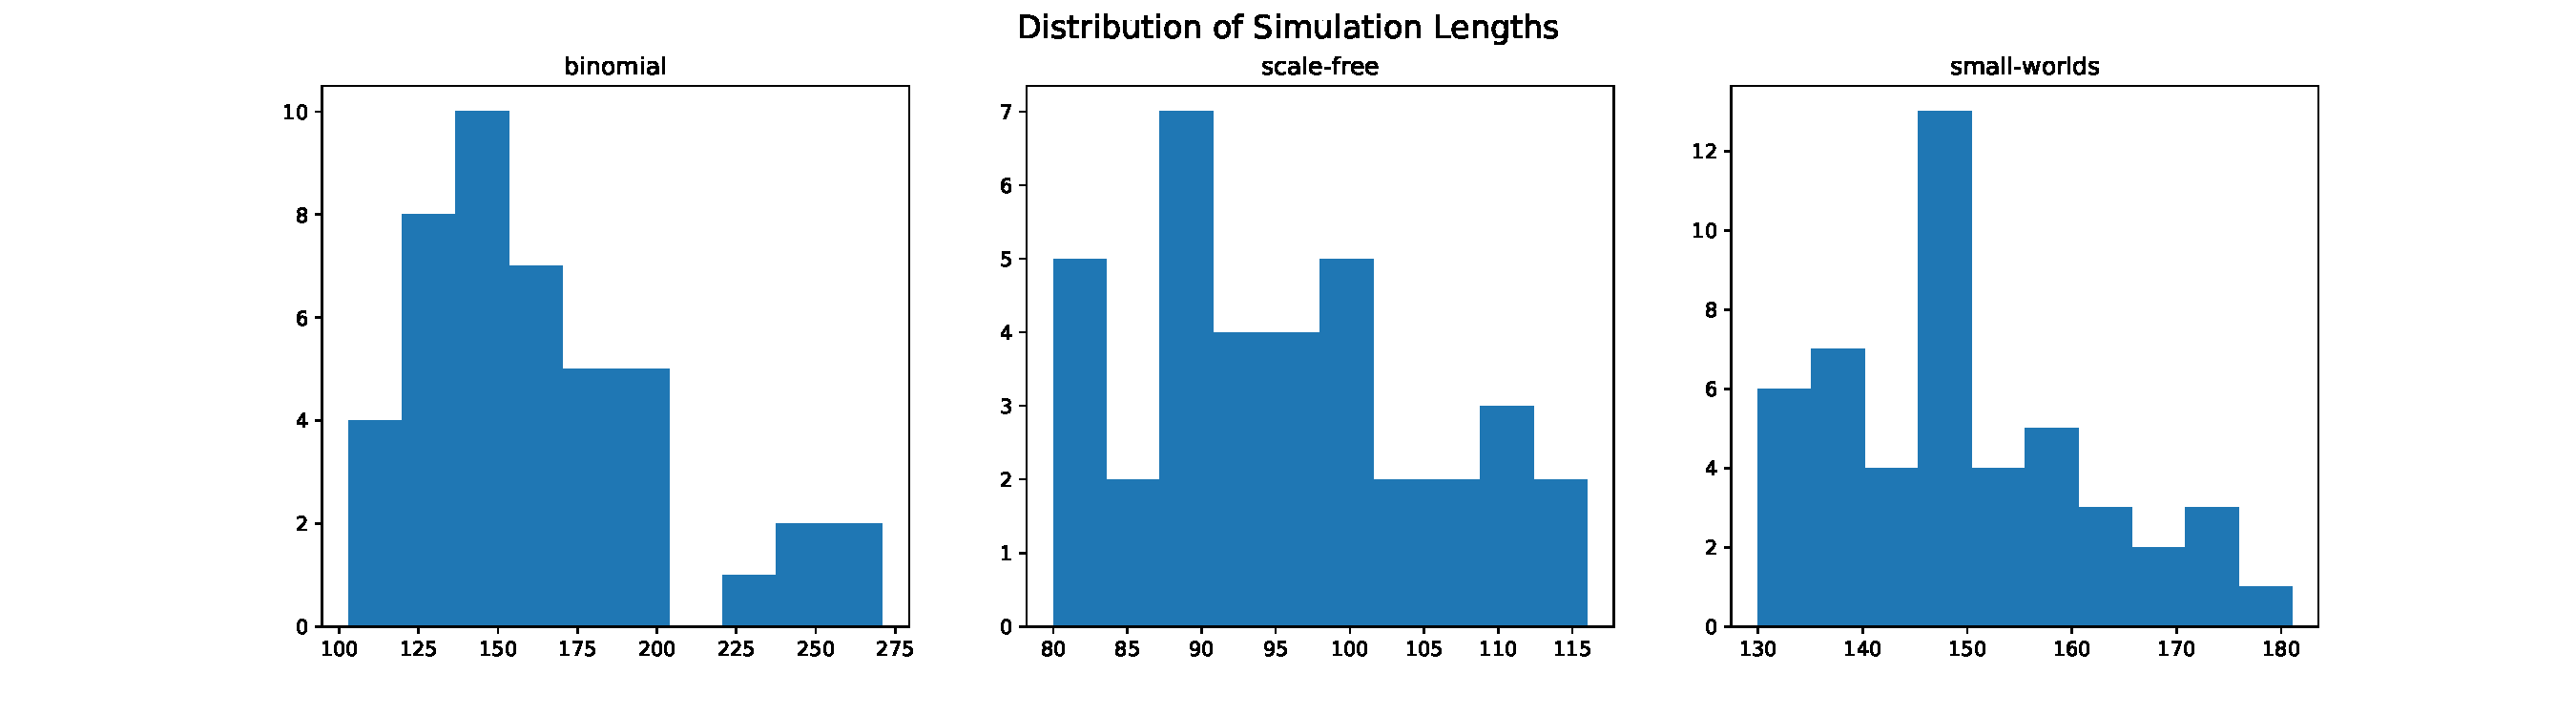
\includegraphics[width=0.5\textwidth]{img/distributions.pdf}
  \end{center}
	\caption{Distribution of simulation lengths across different random seeds and graph instances for each topology with $p_{inf} = p_cure = 0.03$ and graph size (10000,50000). The results show that they show a gaussian-like distribution.}
	\label{fig:normal-dist}
\end{figure}

\section{Results - Program 1}

In this section, we will present some of the main results of Program 1, ie. infection without cure.

\subsection{Comparing Across Infection Probabilities}\label{sec:pg1-compare-pis}

\begin{figure}[htb]
  \begin{center}
	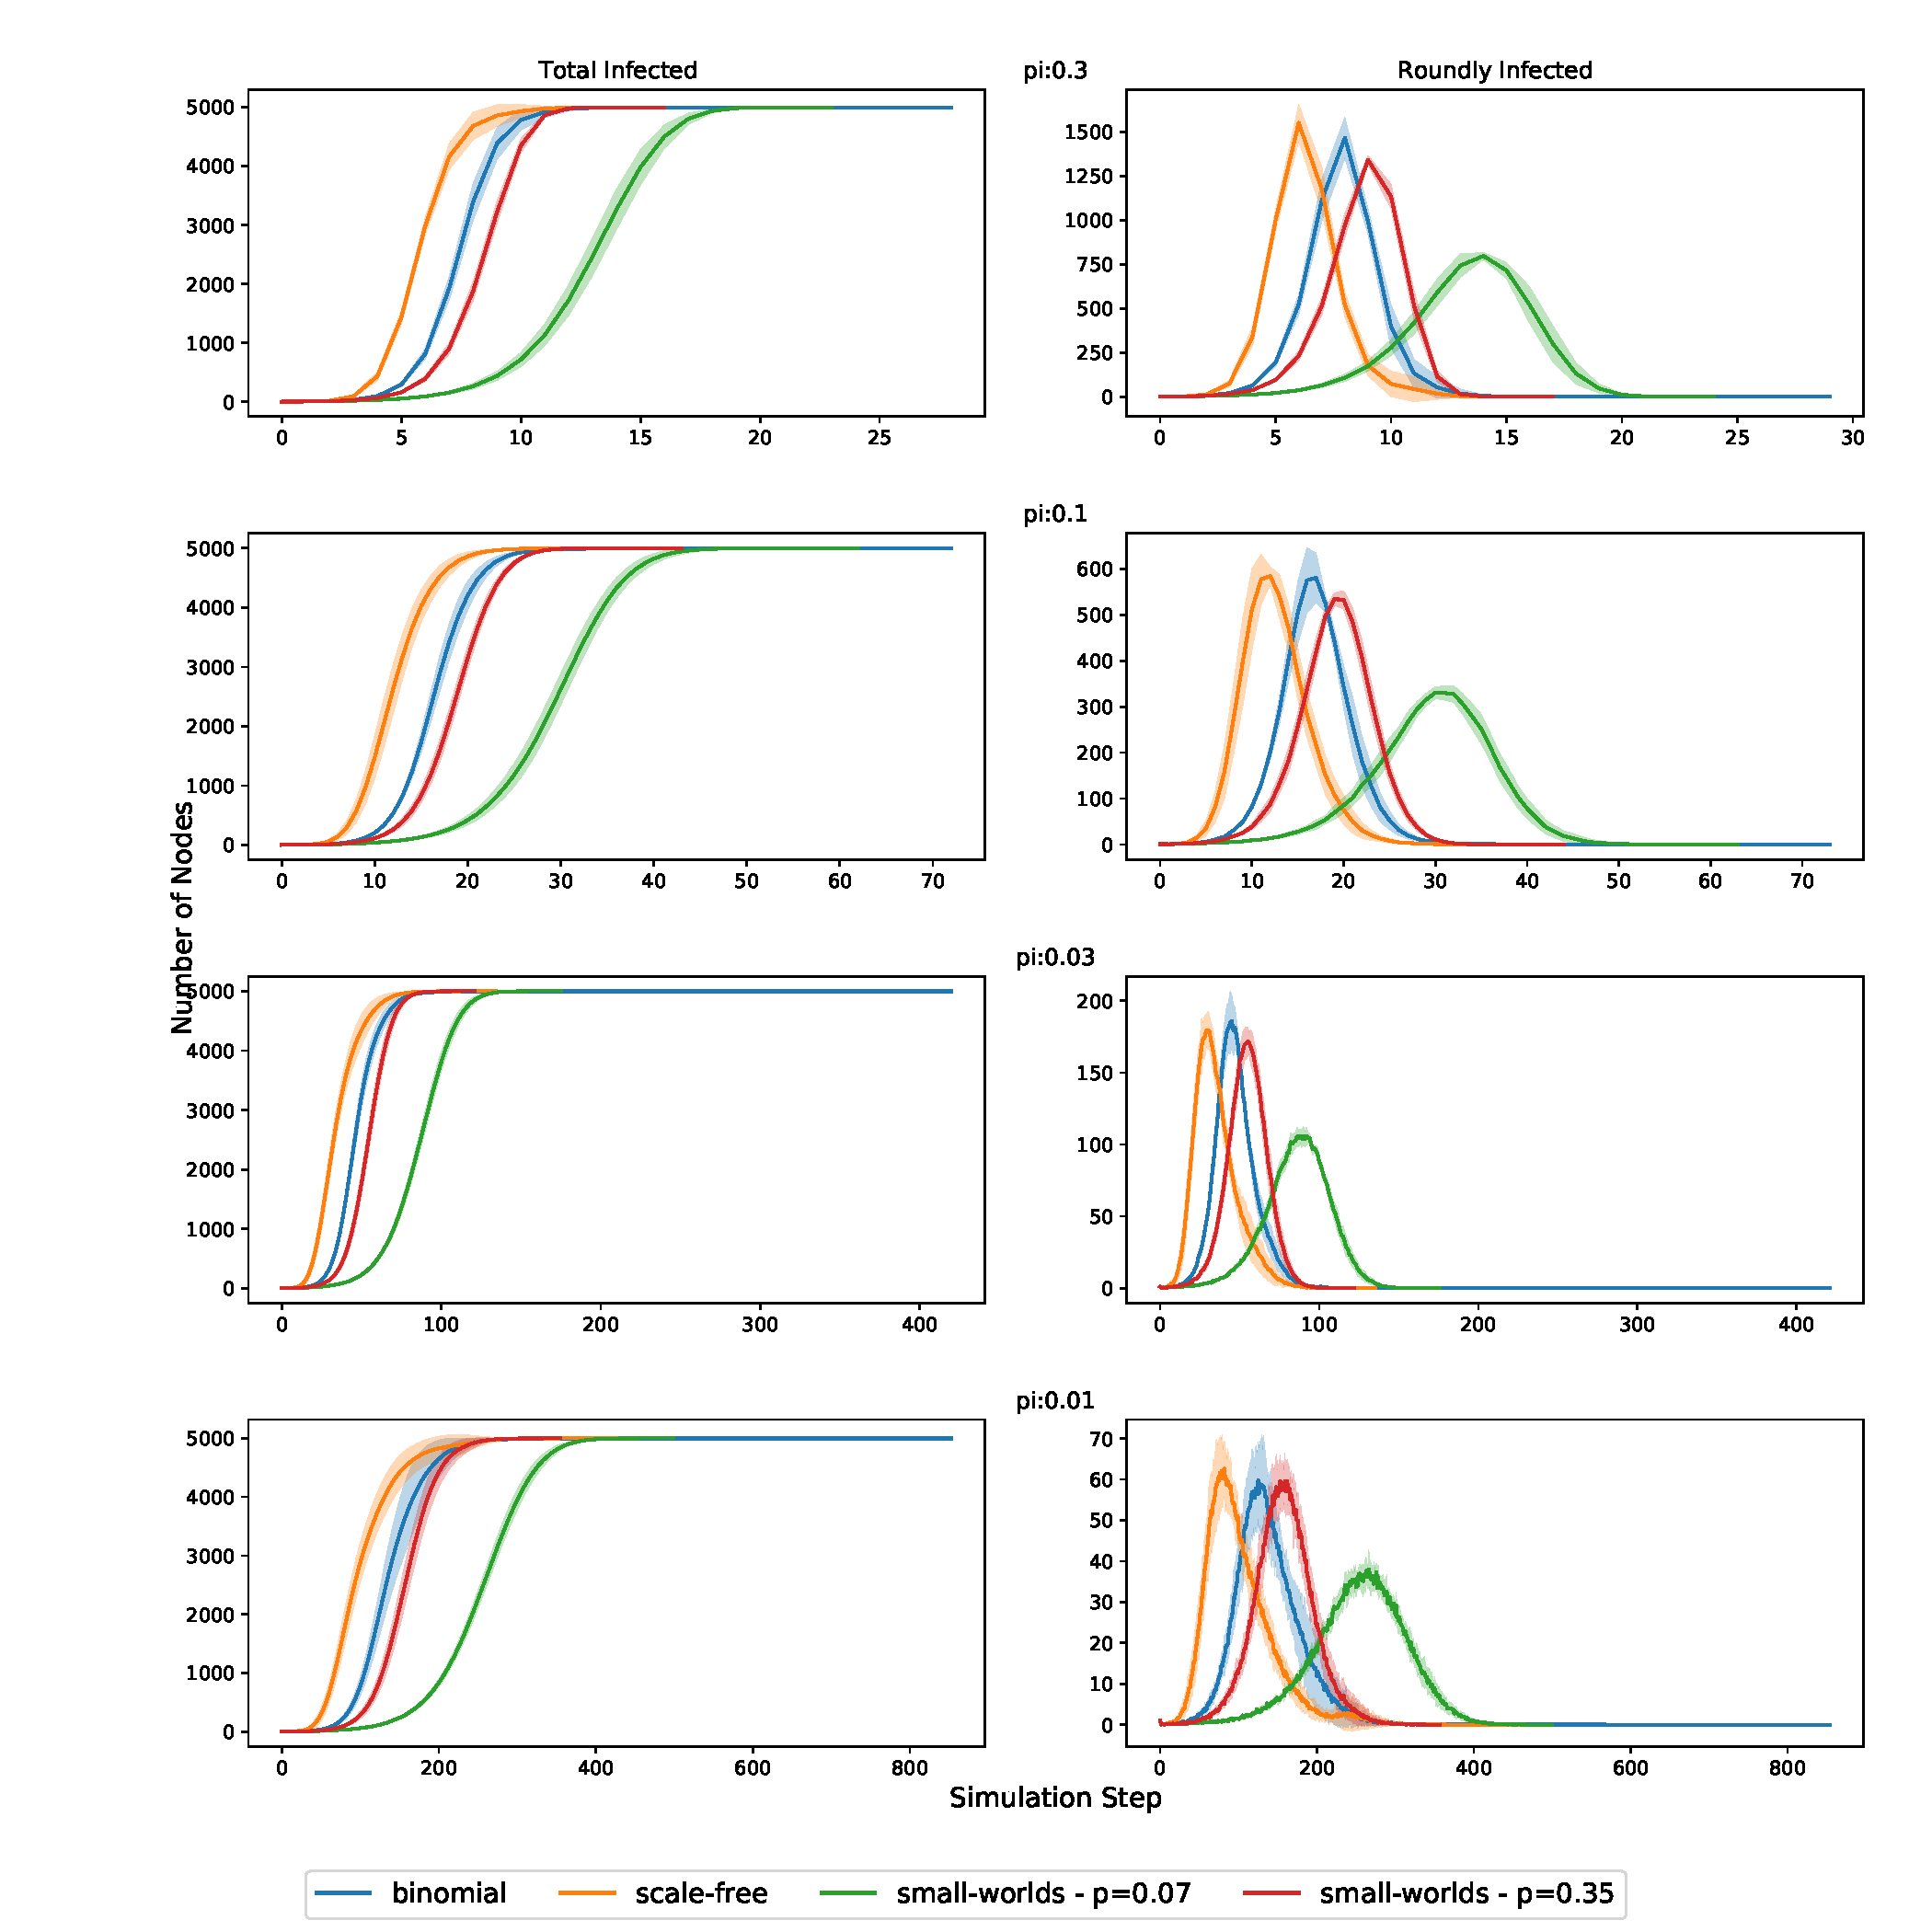
\includegraphics[width=0.5\textwidth]{img/pg1-pis-compare_ms_5k.pdf}
  \end{center}
	\caption{Comparing infection behavior with unlimited resources of different topologies under different infection probabilities. Note that there are two different versions of small-worlds graph: one with rewiring probability 0.07 and other with 0.35. Graphs has 5000 nodes and 20000 edges. Shaded regions show $\pm \sigma$. Note that shaded regions usually not visible, indicating the statistical significance of our results.}
	\label{fig:pg1-pis-compare_ms_5k}
\end{figure}

\autoref{fig:pg1-pis-compare_ms_5k} is our first main result. As can be seen, infection takes shortest time in scale-free graph and longest in small-worlds. A significant observation is that spread in small-worlds graphs gets close to the binomial case as rewiring probability increases. This is expected, as creating shortcuts by rewiring makes small-worlds graphs to lose their distinct character of consisting of "small islands" and get closer to a binomial graph. Due to this behavior, we'll leave out $p_{\text{rewire}}=0.35$ case out in the future graphs for clarity.

As expected, as infection probability decreases, time to infect all nodes increases.

\begin{figure}[htb]
  \begin{center}
	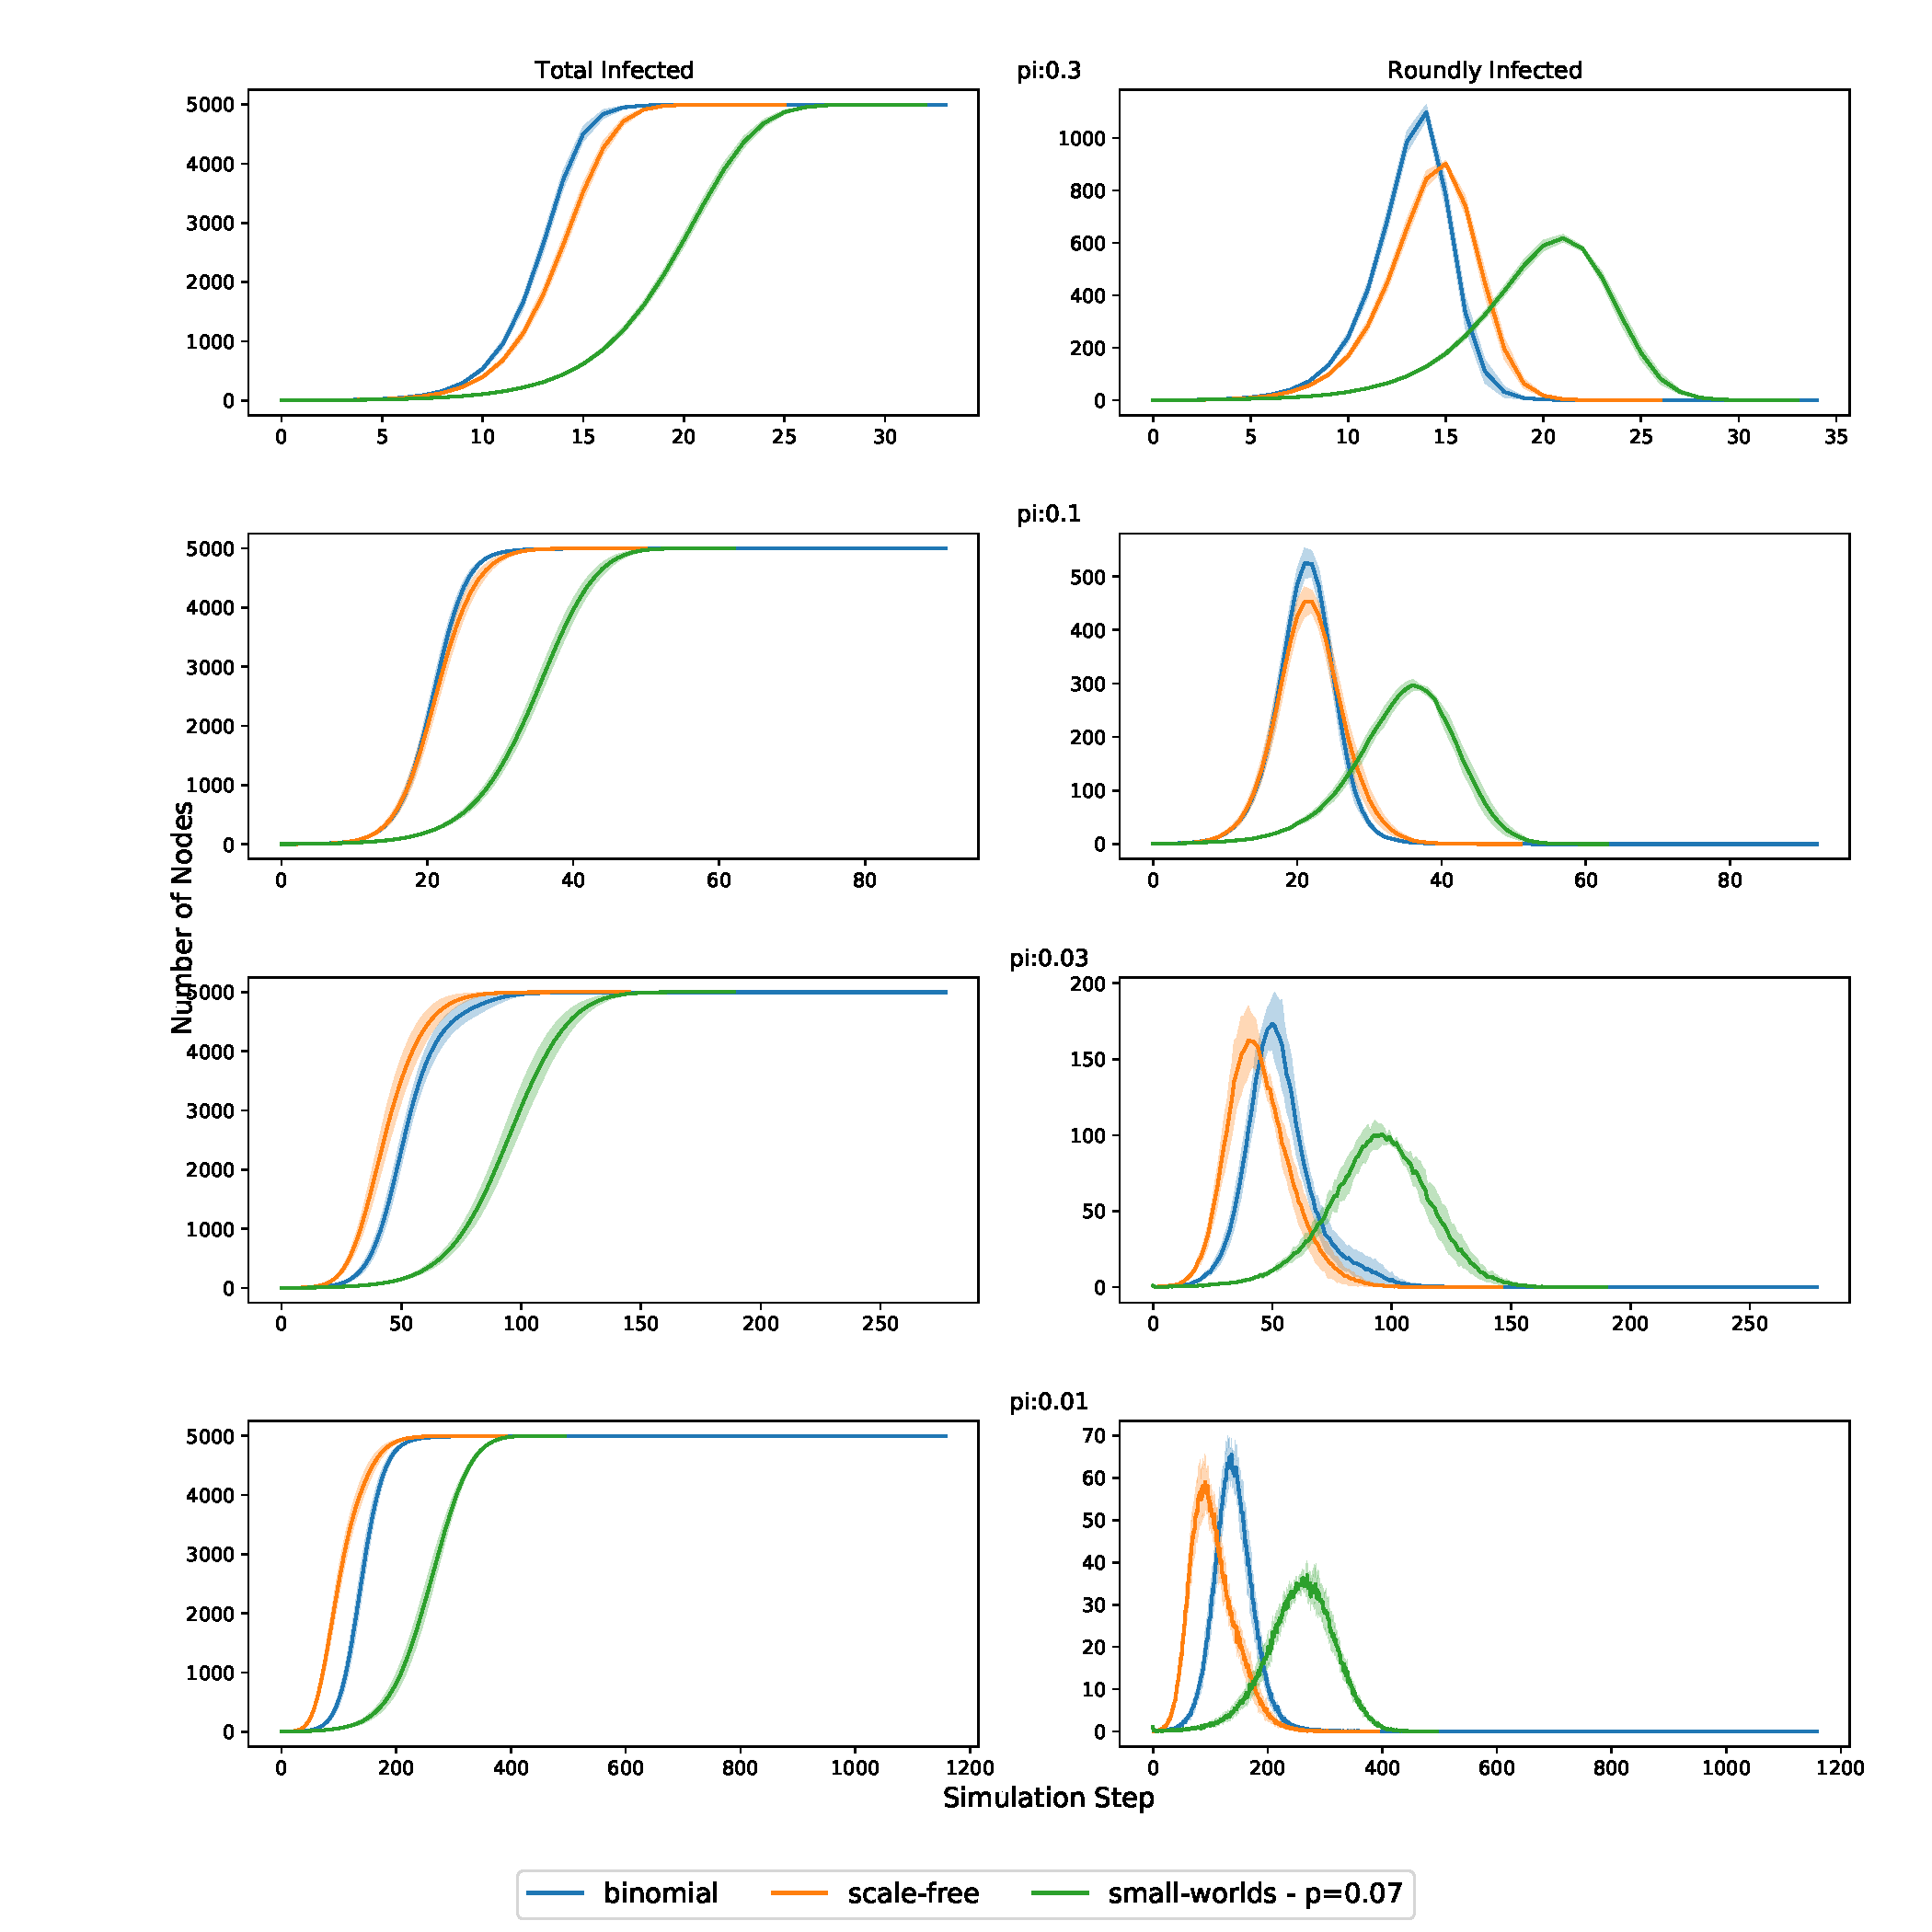
\includegraphics[width=0.5\textwidth]{img/pg1-pis-compare_ss_5k.pdf}
  \end{center}
	\caption{\autoref{fig:pg1-pis-compare_ms_5k} figure but with single infection spread model. Also small-worlds with $p_{\text{rewire}}=0.35$ is left out.}
	\label{fig:pg1-pis-compare_ss_5k}
\end{figure}

Comparing \autoref{fig:pg1-pis-compare_ss_5k} with \autoref{fig:pg1-pis-compare_ms_5k} shows another interesting insight into relation between spread models and graph topologies. For high probabilities of infection, infection spreads faster than scale-free graphs. Because we allow only 1 infection per infected node, no matter their degree, hub nodes actually becomes bottlenecks. They cannot utilize their highly connected status and since we keep the number of edges same across topologies, others part are less connected than a binomial graph.

This effect is not visible for small probabilities because hubs aren't able to infect that many neighbors anyways. In other words, infection probability becomes the bottleneck instead of infection limit.

\begin{figure}[htb]
  \begin{center}
	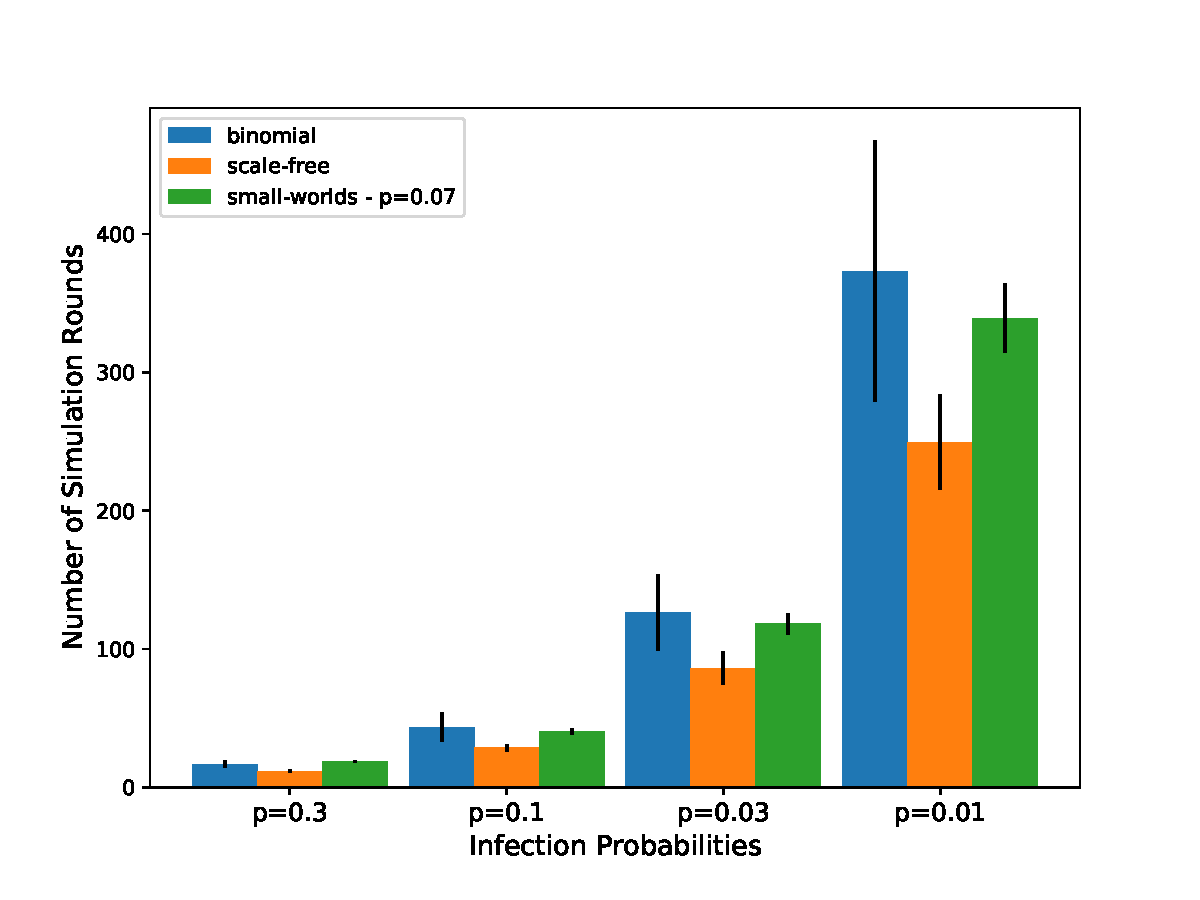
\includegraphics[width=0.5\textwidth]{img/pg1-pis-compare_ms_10k_bar.pdf}
  \end{center}
	\caption{Time to fully infect the network for different infection probabilities and different topologies. Network size is (10000,50000) and unlimited resource spread model is used. Error bars show $\pm \sigma$.}
	\label{fig:pg1-pis-compare_ms_10k_bar}
\end{figure}

\autoref{fig:pg1-pis-compare_ms_10k_bar} shows that while it is not visible from infection curves; in fact it takes longer for binomial networks to be fully infected. The reasons will be discussed in \autoref{sec:binomial takes longest}.

\subsection{Comparing Across Graph Sizes}


\begin{figure}[htb]
  \begin{center}
	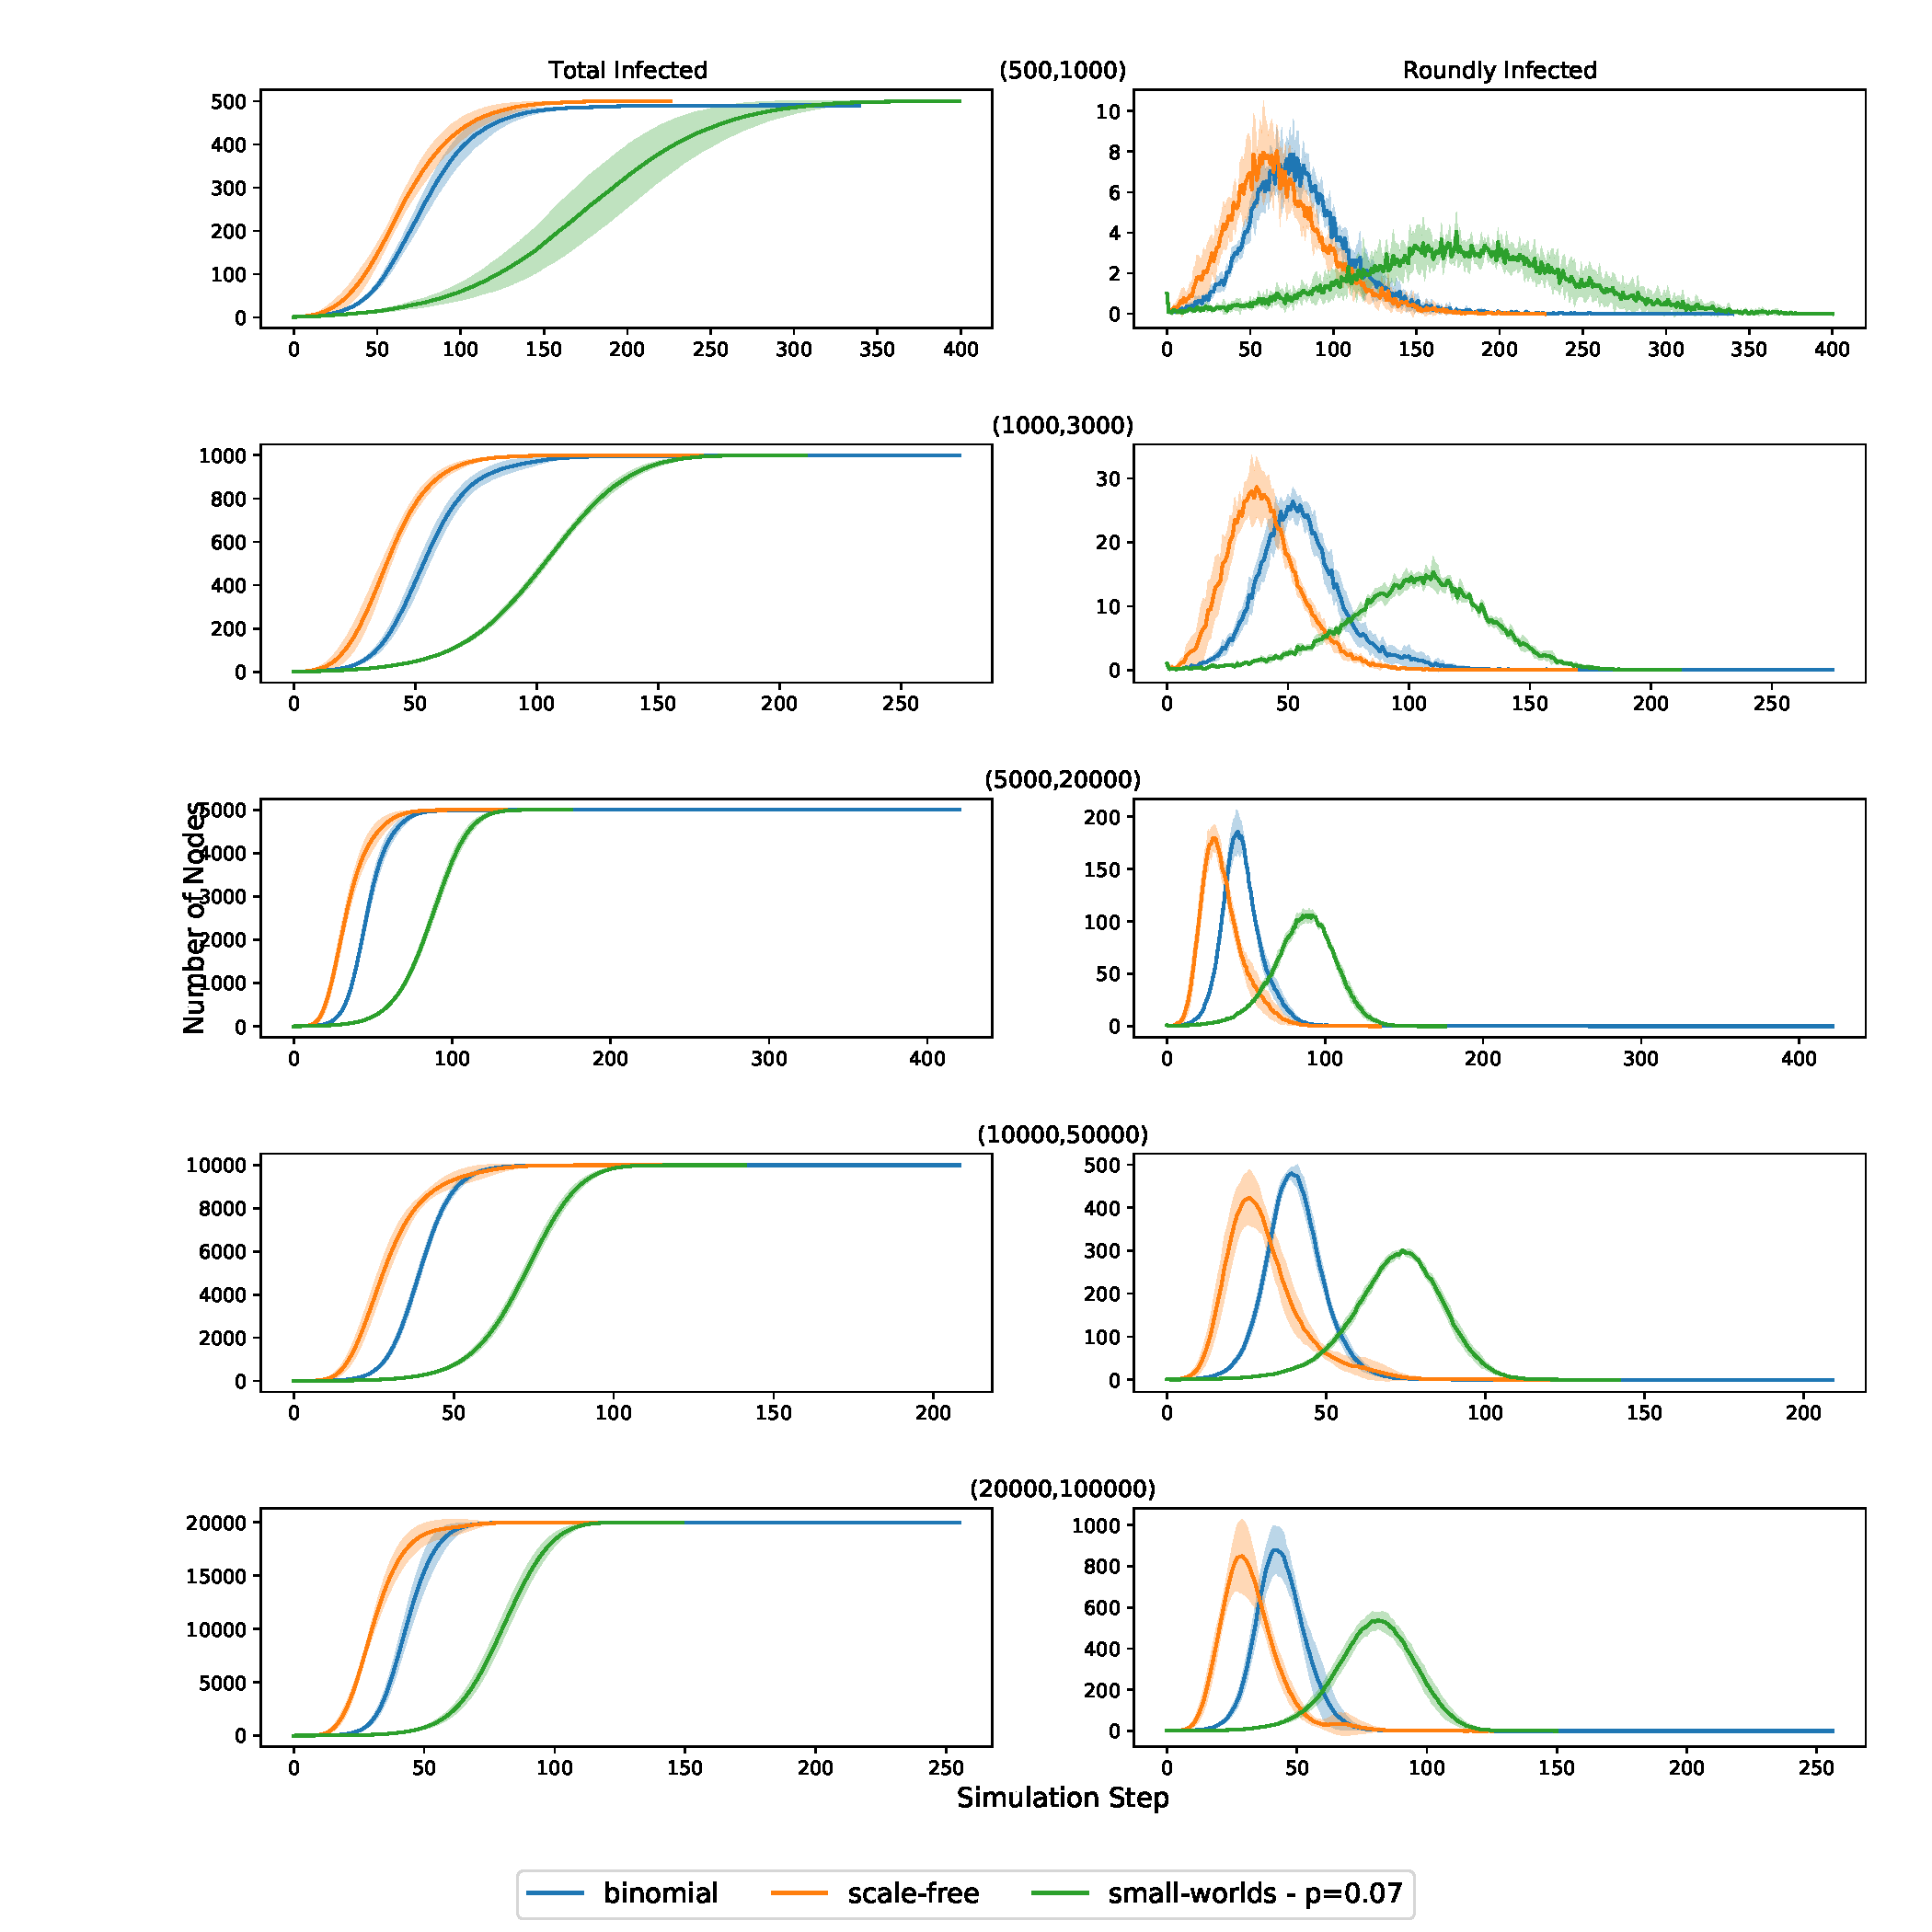
\includegraphics[width=0.5\textwidth]{img/pg1-sizes-compare_ms_p003.pdf}
  \end{center}
	\caption{Comparison of infection rates on graphs of different sizes. All figures use $p_{inf} = 0.03$ and unlimited spread model.}
	\label{fig:pg1-sizes-compare_ms_p003}
\end{figure}

\begin{figure}[htb]
  \begin{center}
	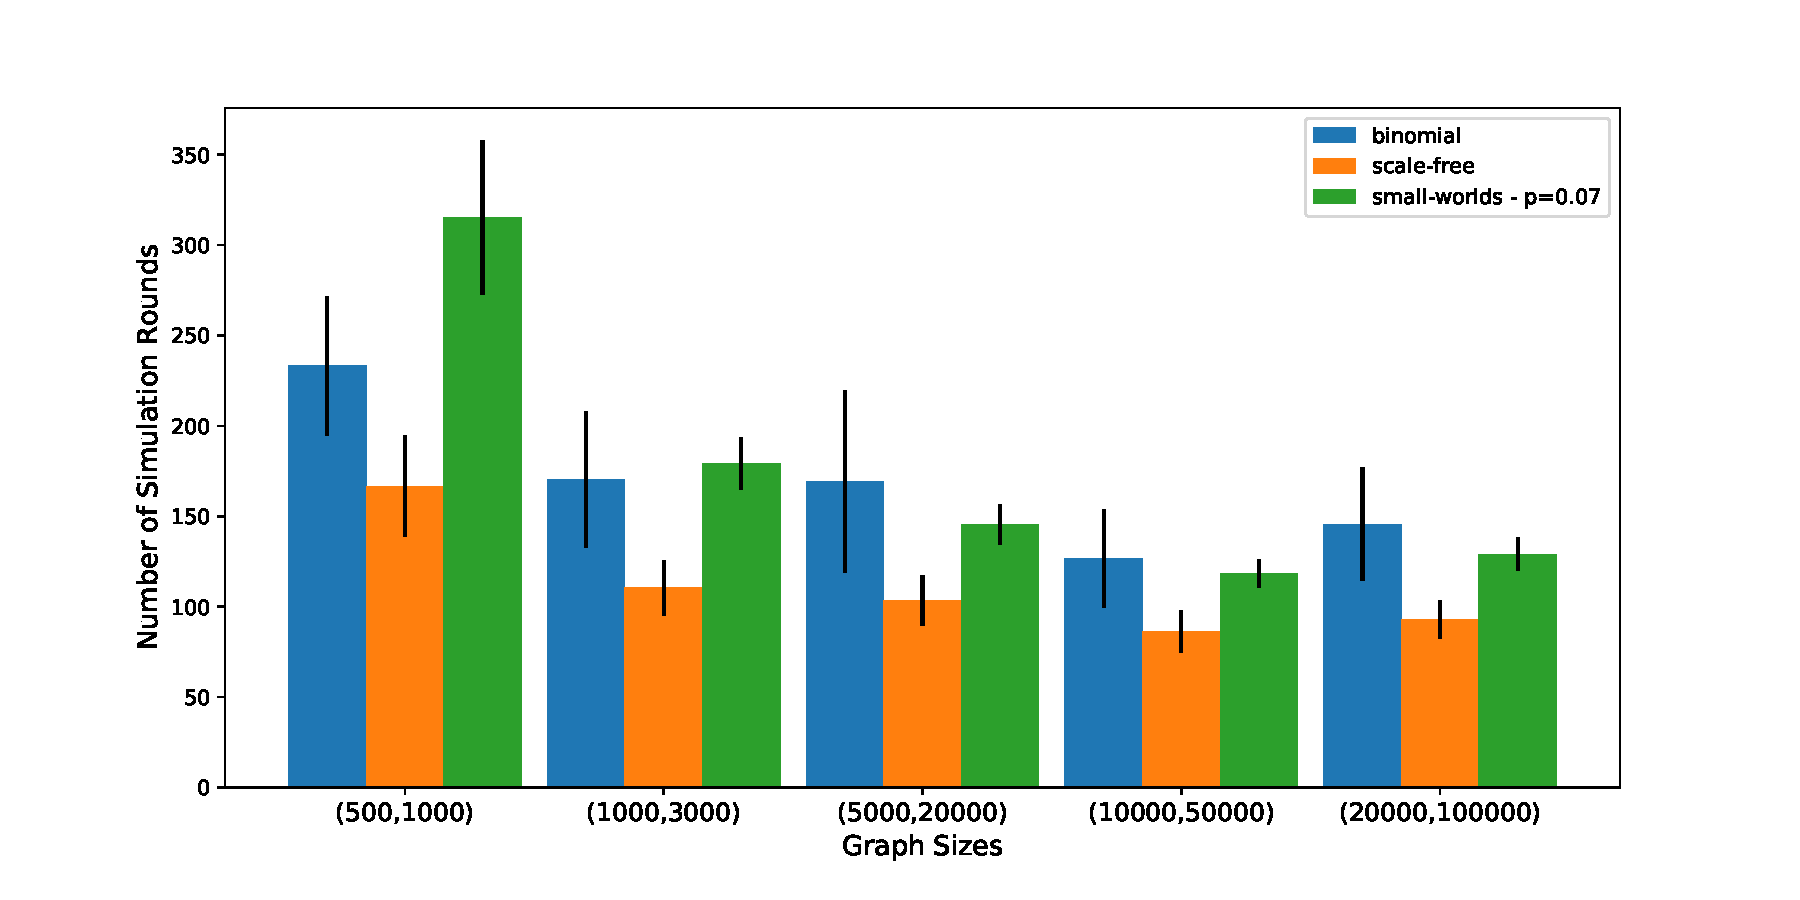
\includegraphics[width=0.5\textwidth]{img/pg1-sizes-compare_ms_003_bar.pdf}
  \end{center}
	\caption{Time to completely infect the network. All figures use $p_{inf} = 0.03$ and unlimited spread model. Error bars show $\pm \sigma$.}
	\label{fig:pg1-sizes-compare_ms_003_bar}
\end{figure}

\autoref{fig:pg1-sizes-compare_ms_p003} and \autoref{fig:pg1-sizes-compare_ms_003_bar} show that the comparison between different topologies holds across different network sizes for large networks.

An interesting observation is that average degree is a much more important metric than the network size when comparing time to infect a network.

While increasing network size while holding average degree slightly increases time to fully infect, as can be seen by comparing $(10000,50000)$ and $(20000,100000)$; the smaller networks has much higher time to fully infect because of their smaller average degree. This suggests that infection spread scales really well.

Note that for the smallest networks, binomial takes shorter to fully infect than small-worlds. This will be addressed in \autoref{sec:binomial takes longest}.



\section{Results - Program 2}\label{sec:pg2-res}

In this section, we will present some of the main results of Program 2, ie. when a cure is introduced.

\subsection{Introducing A Cure}

\begin{figure}[htb]
  \begin{center}
	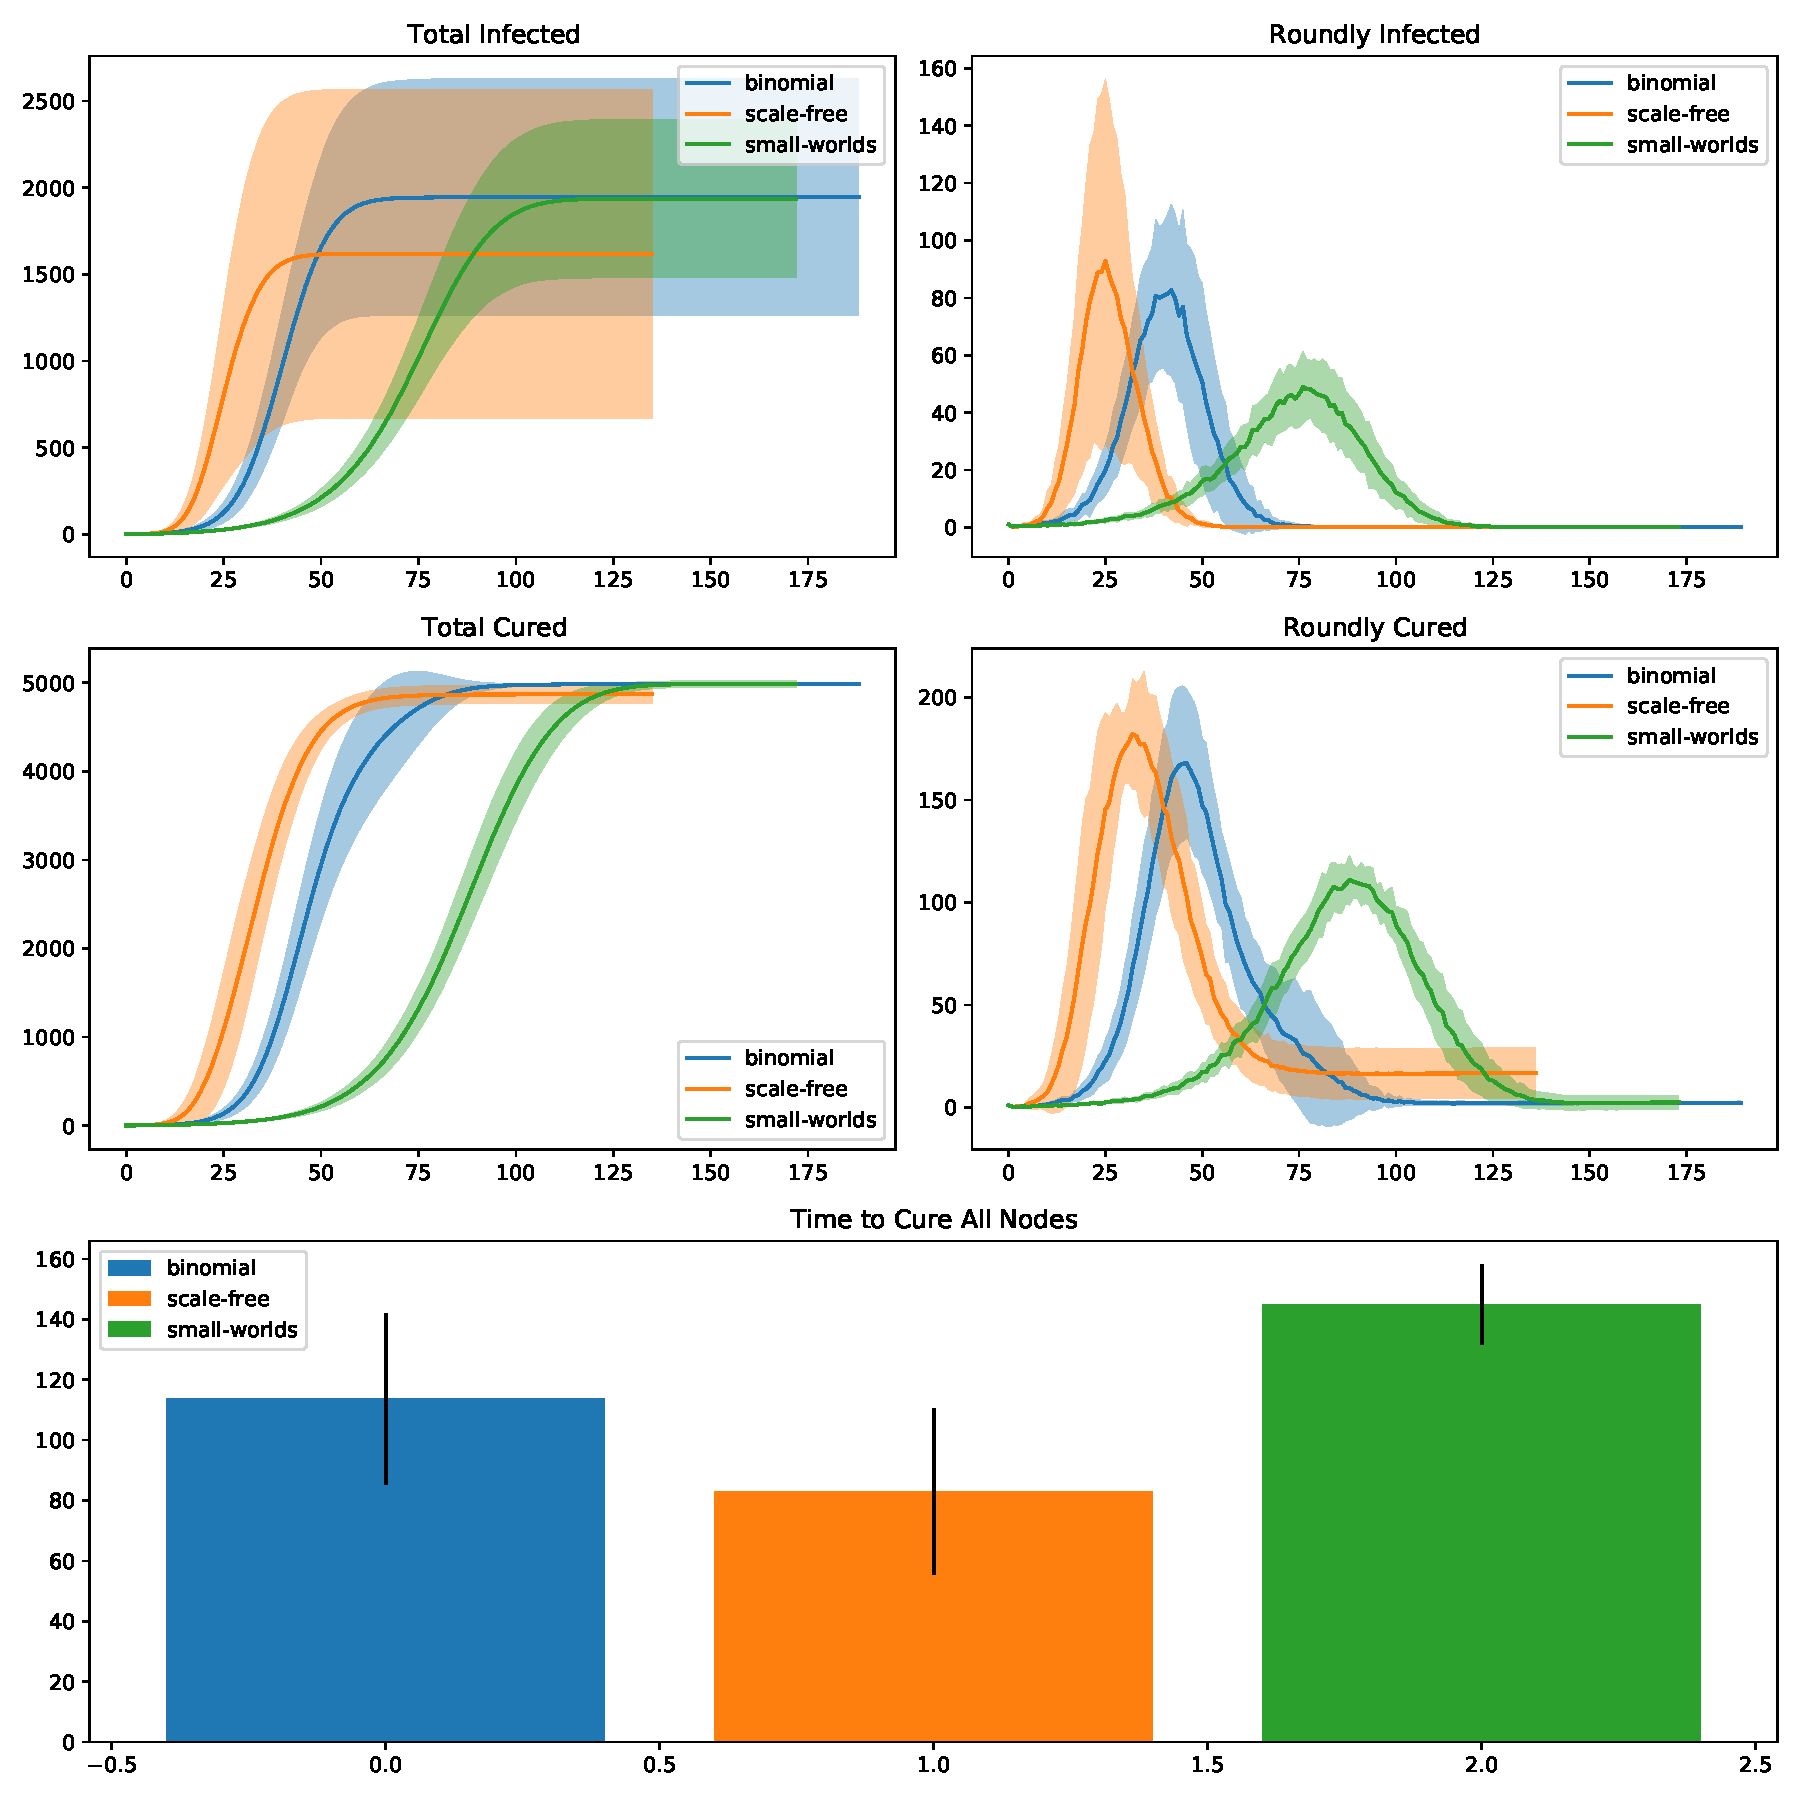
\includegraphics[width=0.5\textwidth]{img/pg2-5000_20000_ms_p003.pdf}
  \end{center}
	\caption{Example simulation results when a cure is introduced. Graph size (5000,20000) and $p_{inf} = p_{cure} = 0.03$.}
	\label{fig:pg2-5000_20000_ms_p003}
\end{figure}

\autoref{fig:pg2-5000_20000_ms_p003} is provided to show how simulation unfolds. As our analysis focus on infection rates, total and roundly cured results will be omitted in the future figures.
Notice that total infection figure still has the S-shape. This is because we count previously infected but cured nodes too, following the convention of \cite{redcode}.

\subsection{With Cure vs Without Cure}\label{sec:one2one-cure}

\begin{figure}[htb]
  \begin{center}
	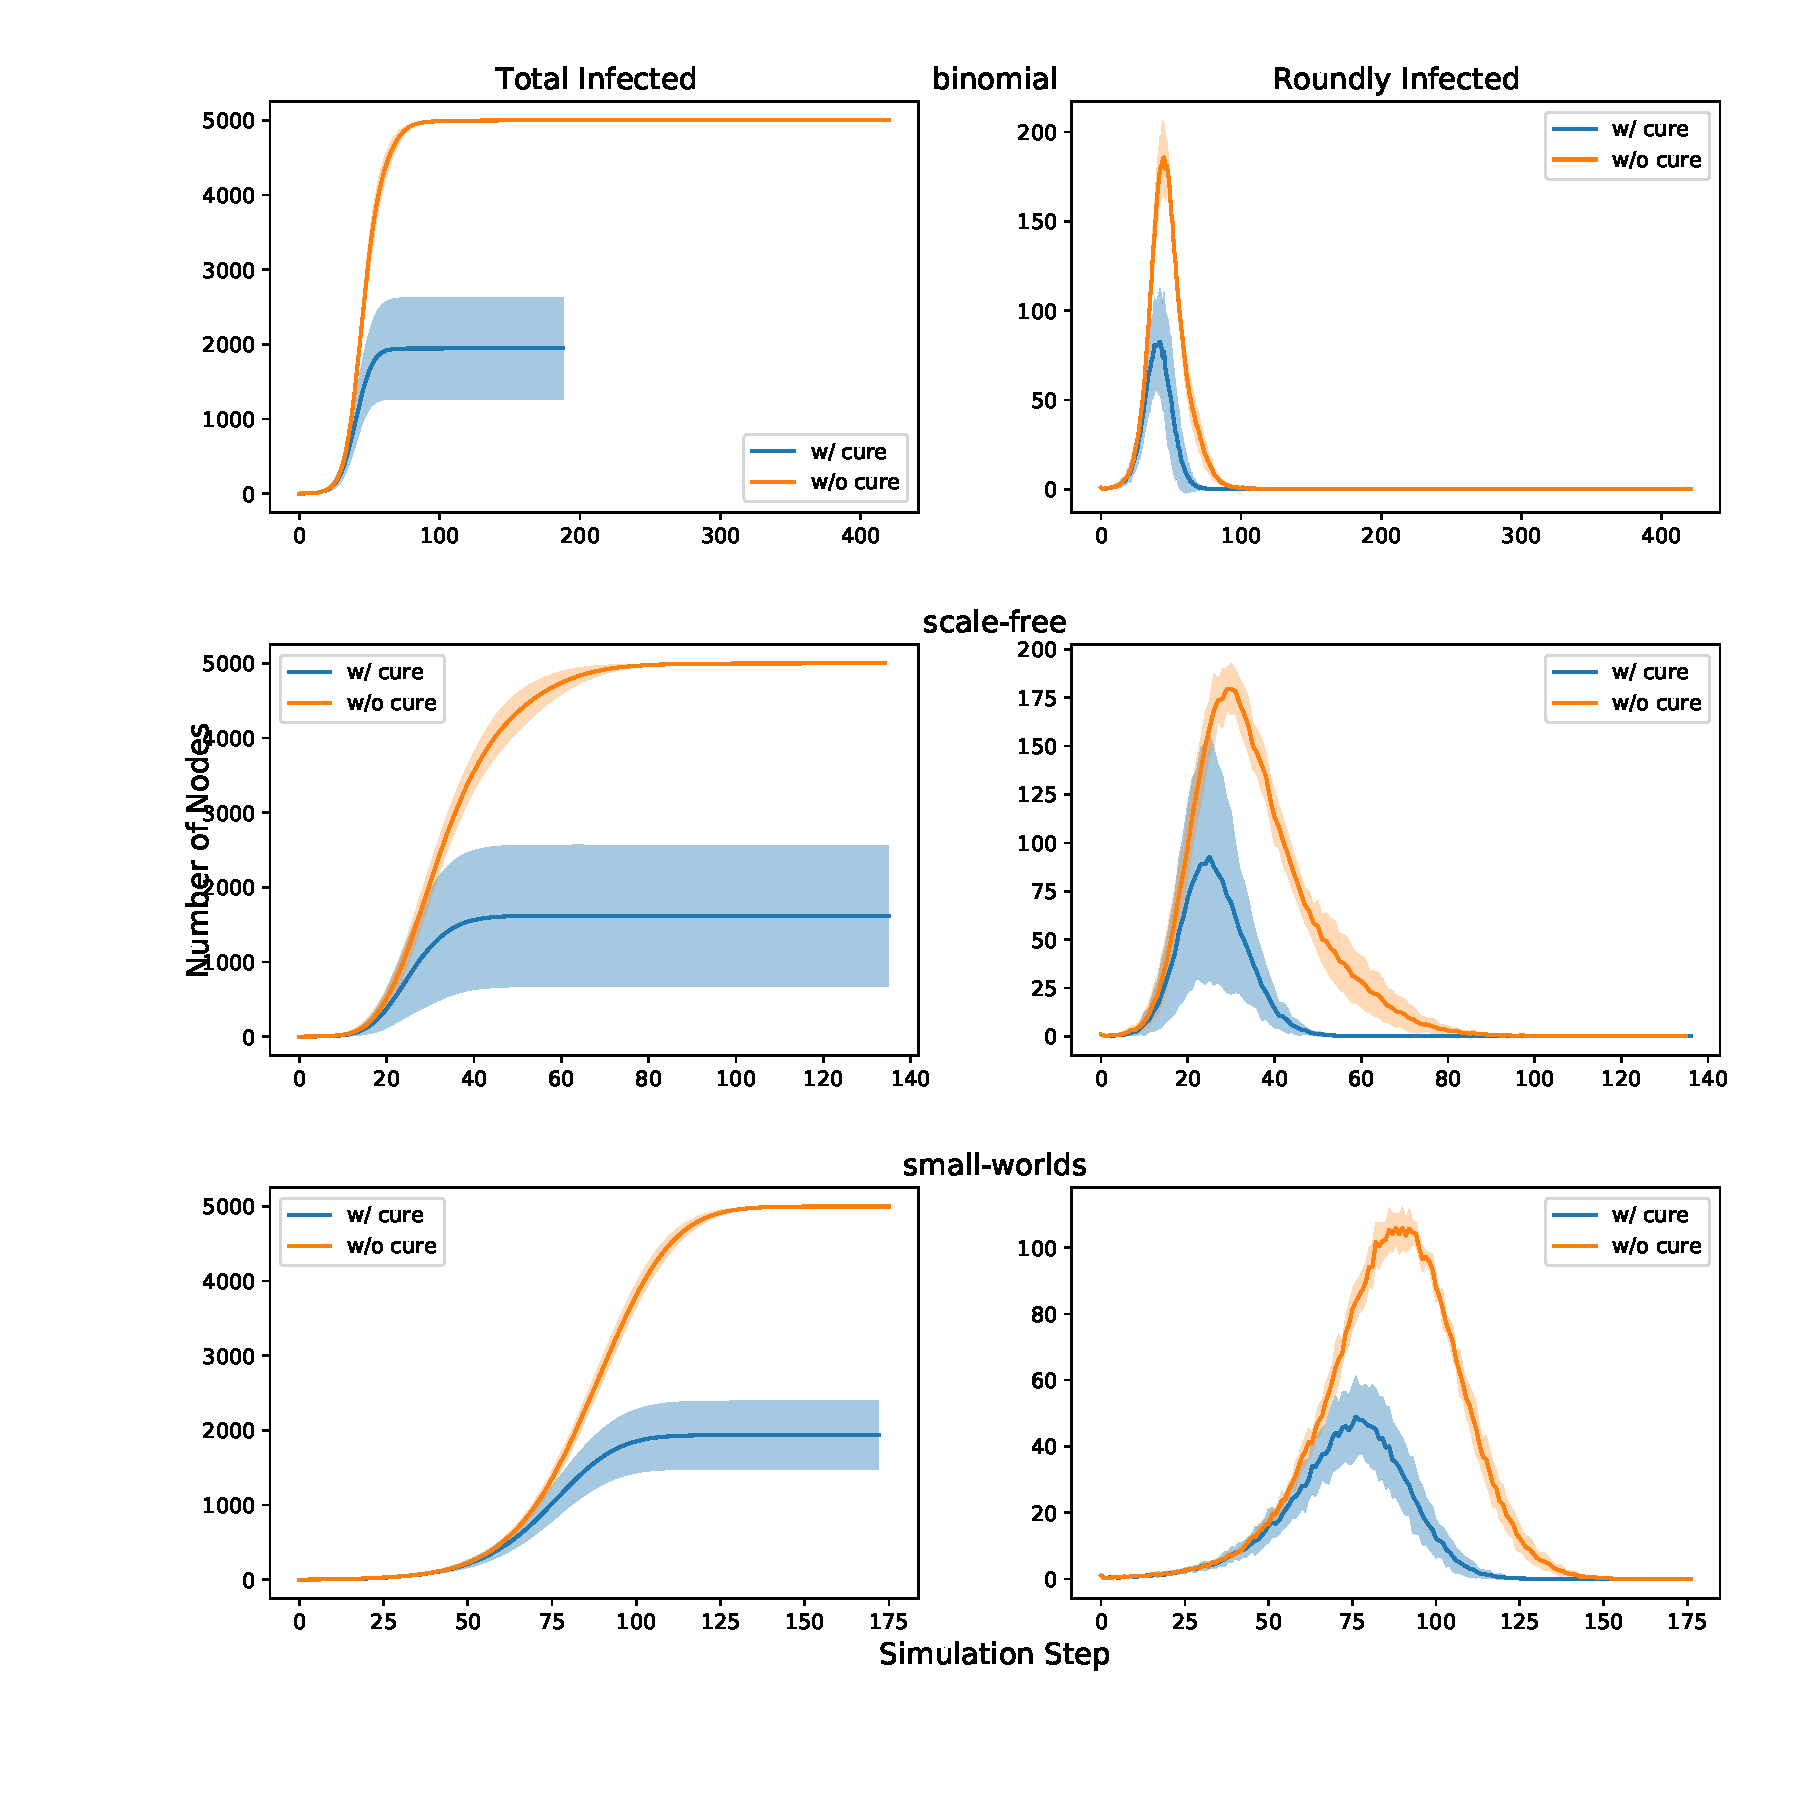
\includegraphics[width=0.5\textwidth]{img/pg2-one2one-5000_20000_ms_p003.pdf}
  \end{center}
	\caption{A comparison of w/ cure and w/o cure spreads across different topologies. Graph size (5000,20000) and $p_{inf} = p_{cure} = 0.03$.}
	\label{fig:pg2-one2one-5000_20000_ms_p003}
\end{figure}

\autoref{fig:pg2-one2one-5000_20000_ms_p003} shows how introducing a cure affects the infection spread. As expected, it reduces number of infected nodes. In the next two sections, we will see how varying infection probabilities and graph sizes affect this difference.

\subsection{Compare Across Different Infection Probabilities}\label{sec:pg2-compares-pis}

\begin{figure}[htb]
  \begin{center}
	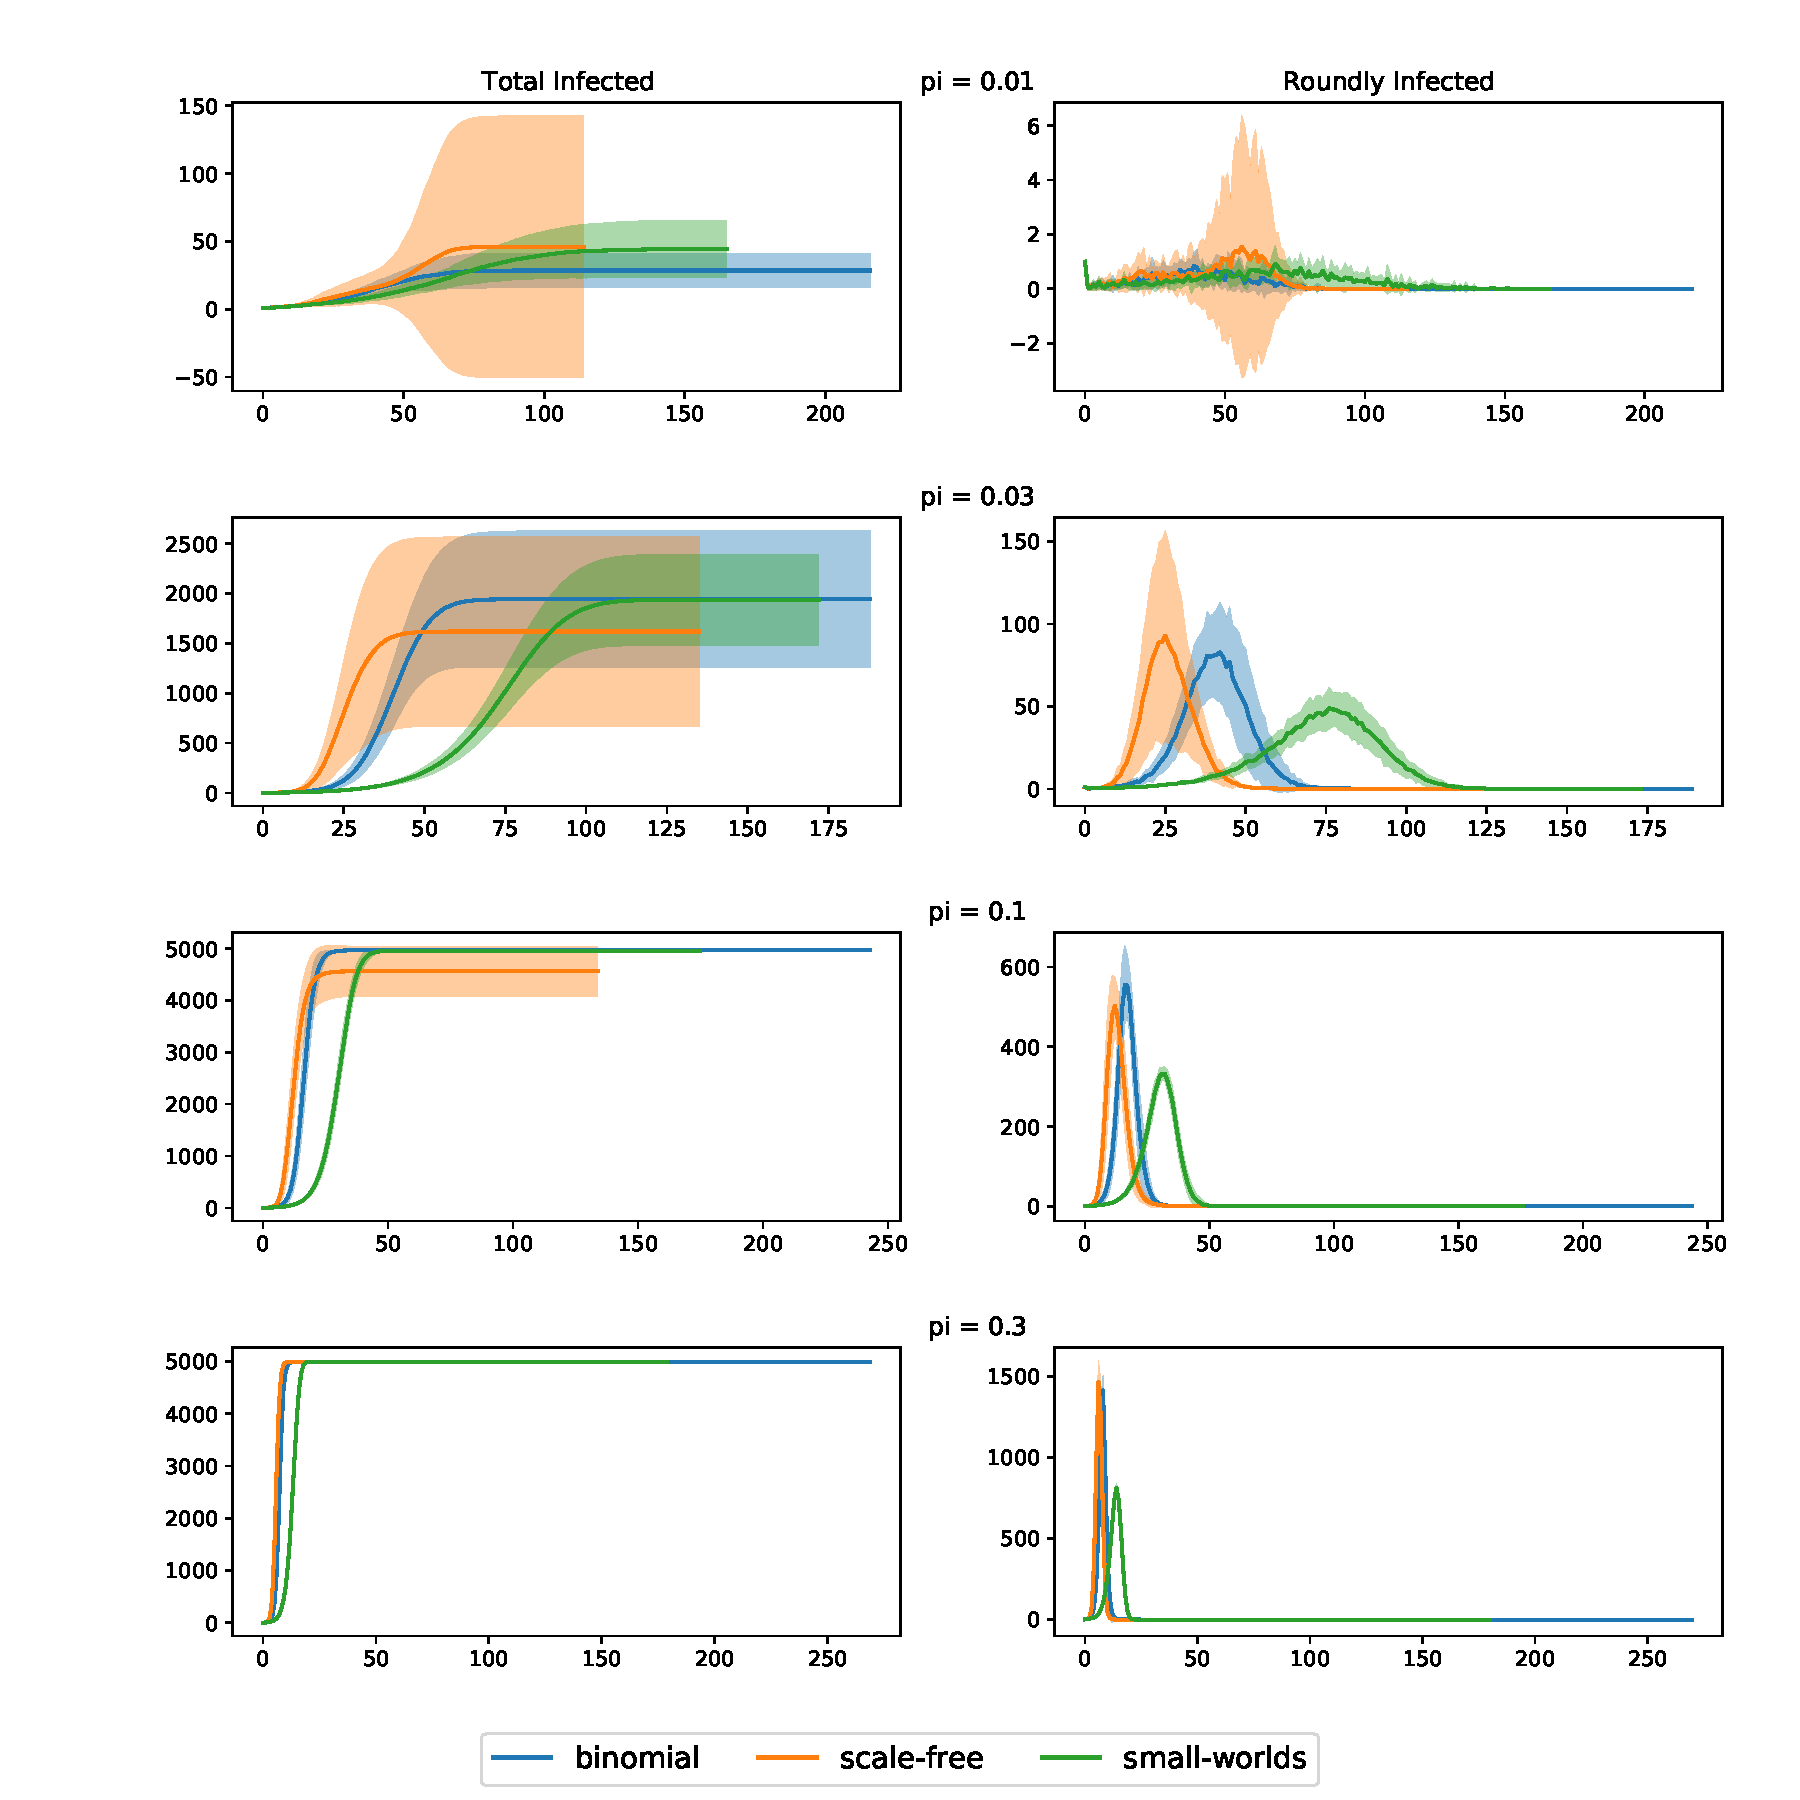
\includegraphics[width=0.5\textwidth]{img/pg2-pis-compare_ms_5k.pdf}
  \end{center}
	\caption{Comparing infection behavior with unlimited resources of different topologies under different infection probabilities when there is a cure. Graph  size is $(5000,20000)$. Shaded regions show $\pm \sigma$.Network size is (5000,20000) and unlimited resource spread model is used. Cure spread probability is always $p_{cure} = 0.03$.}
	\label{fig:pg2-pis-compare_ms_5k}
\end{figure}

\autoref{fig:pg2-pis-compare_ms_5k} show that scale-free networks end the epidemic fastest and usually fewer nodes get infected. However, variance is much higher than other topologies; suggesting the variance is high across different instances and simulation runs. We believe that the differences are due to how soon hub nodes get infected.

Also note that while networks have 5000 nodes, for low infection probability only a portion of them get infected at all. This happens because the cure spread immunizes nodes and severely reduces spread of infection. However, when infection probability is high, infection spreads faster than cure and weakens this effect.


\begin{figure}[htb]
  \begin{center}
	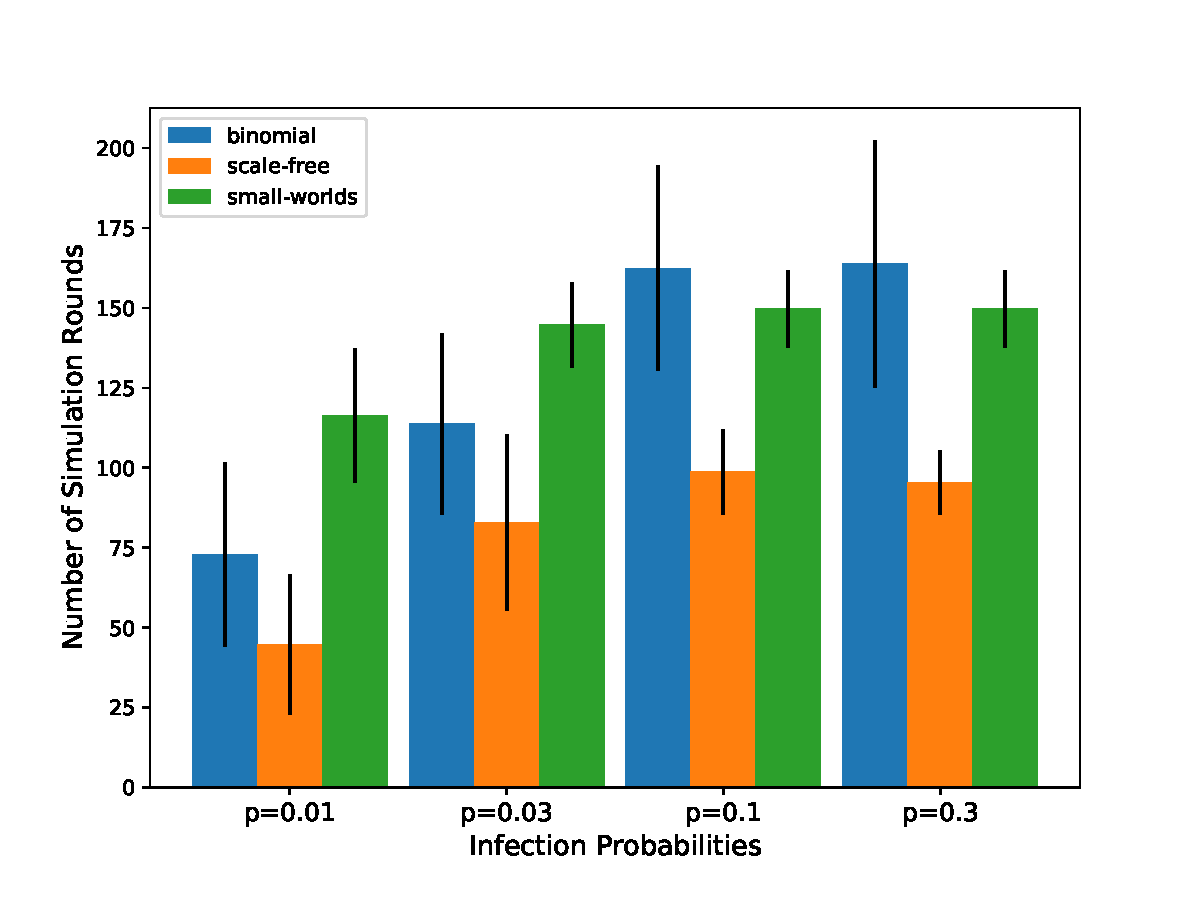
\includegraphics[width=0.5\textwidth]{img/pg2-pis-compare_ms_5k_bar.pdf}
  \end{center}
	\caption{Time to fully infect the network for different infection probabilities and different topologies. Network size is (5000,20000) and unlimited resource spread model is used. Cure spread probability is always $p_{cure} = 0.03$.}
	\label{fig:pg2-pis-compare_ms_5k_bar}
\end{figure}

\autoref{fig:pg2-pis-compare_ms_5k_bar} shows a similar pattern with \autoref{fig:pg1-pis-compare_ms_10k_bar} for high infection probabilities; as in these cases impact of the cure is very small.

However, for small infection probabilities; simulation ends earlier in binomial networks than small-worlds networks, in contrast to \autoref{fig:pg1-pis-compare_ms_10k_bar}. We believe that this happens because having a cure solves "parts of network with very small connectivity" problem of binomial networks. Since the epidemic ends when there aren't any infected nodes but not when everyone cured; there is no need for cure to spread to small-connectivity regions of binomial graphs. This claim is supported by the fact that in $p_{inf} = 0.01$ case; significantly fewer nodes are infected at all in binomial networks than small-worlds networks.


An important observation is in variance is much higher when cure is introduced. While this could be attributed to the changed experiment setup, which uses more instances of networks and fewer runs on the same graph, the results for $p_{inf} = 0.3$ in \autoref{fig:pg2-pis-compare_ms_5k} suggest otherwise. In \autoref{fig:pg1-pis-compare_ms_5k} standard deviations are similar across different infection probabilities; however, they significantly reduce in \autoref{fig:pg2-pis-compare_ms_5k} when infection probability increases. This indicate that the high variance is caused by the stochasticity of how "smartly" the cure will spread because we don't see this when infection probability is high, removing impacts of cure.

\subsection{Compare Across Graph Sizes}


\begin{figure}[htb]
  \begin{center}
	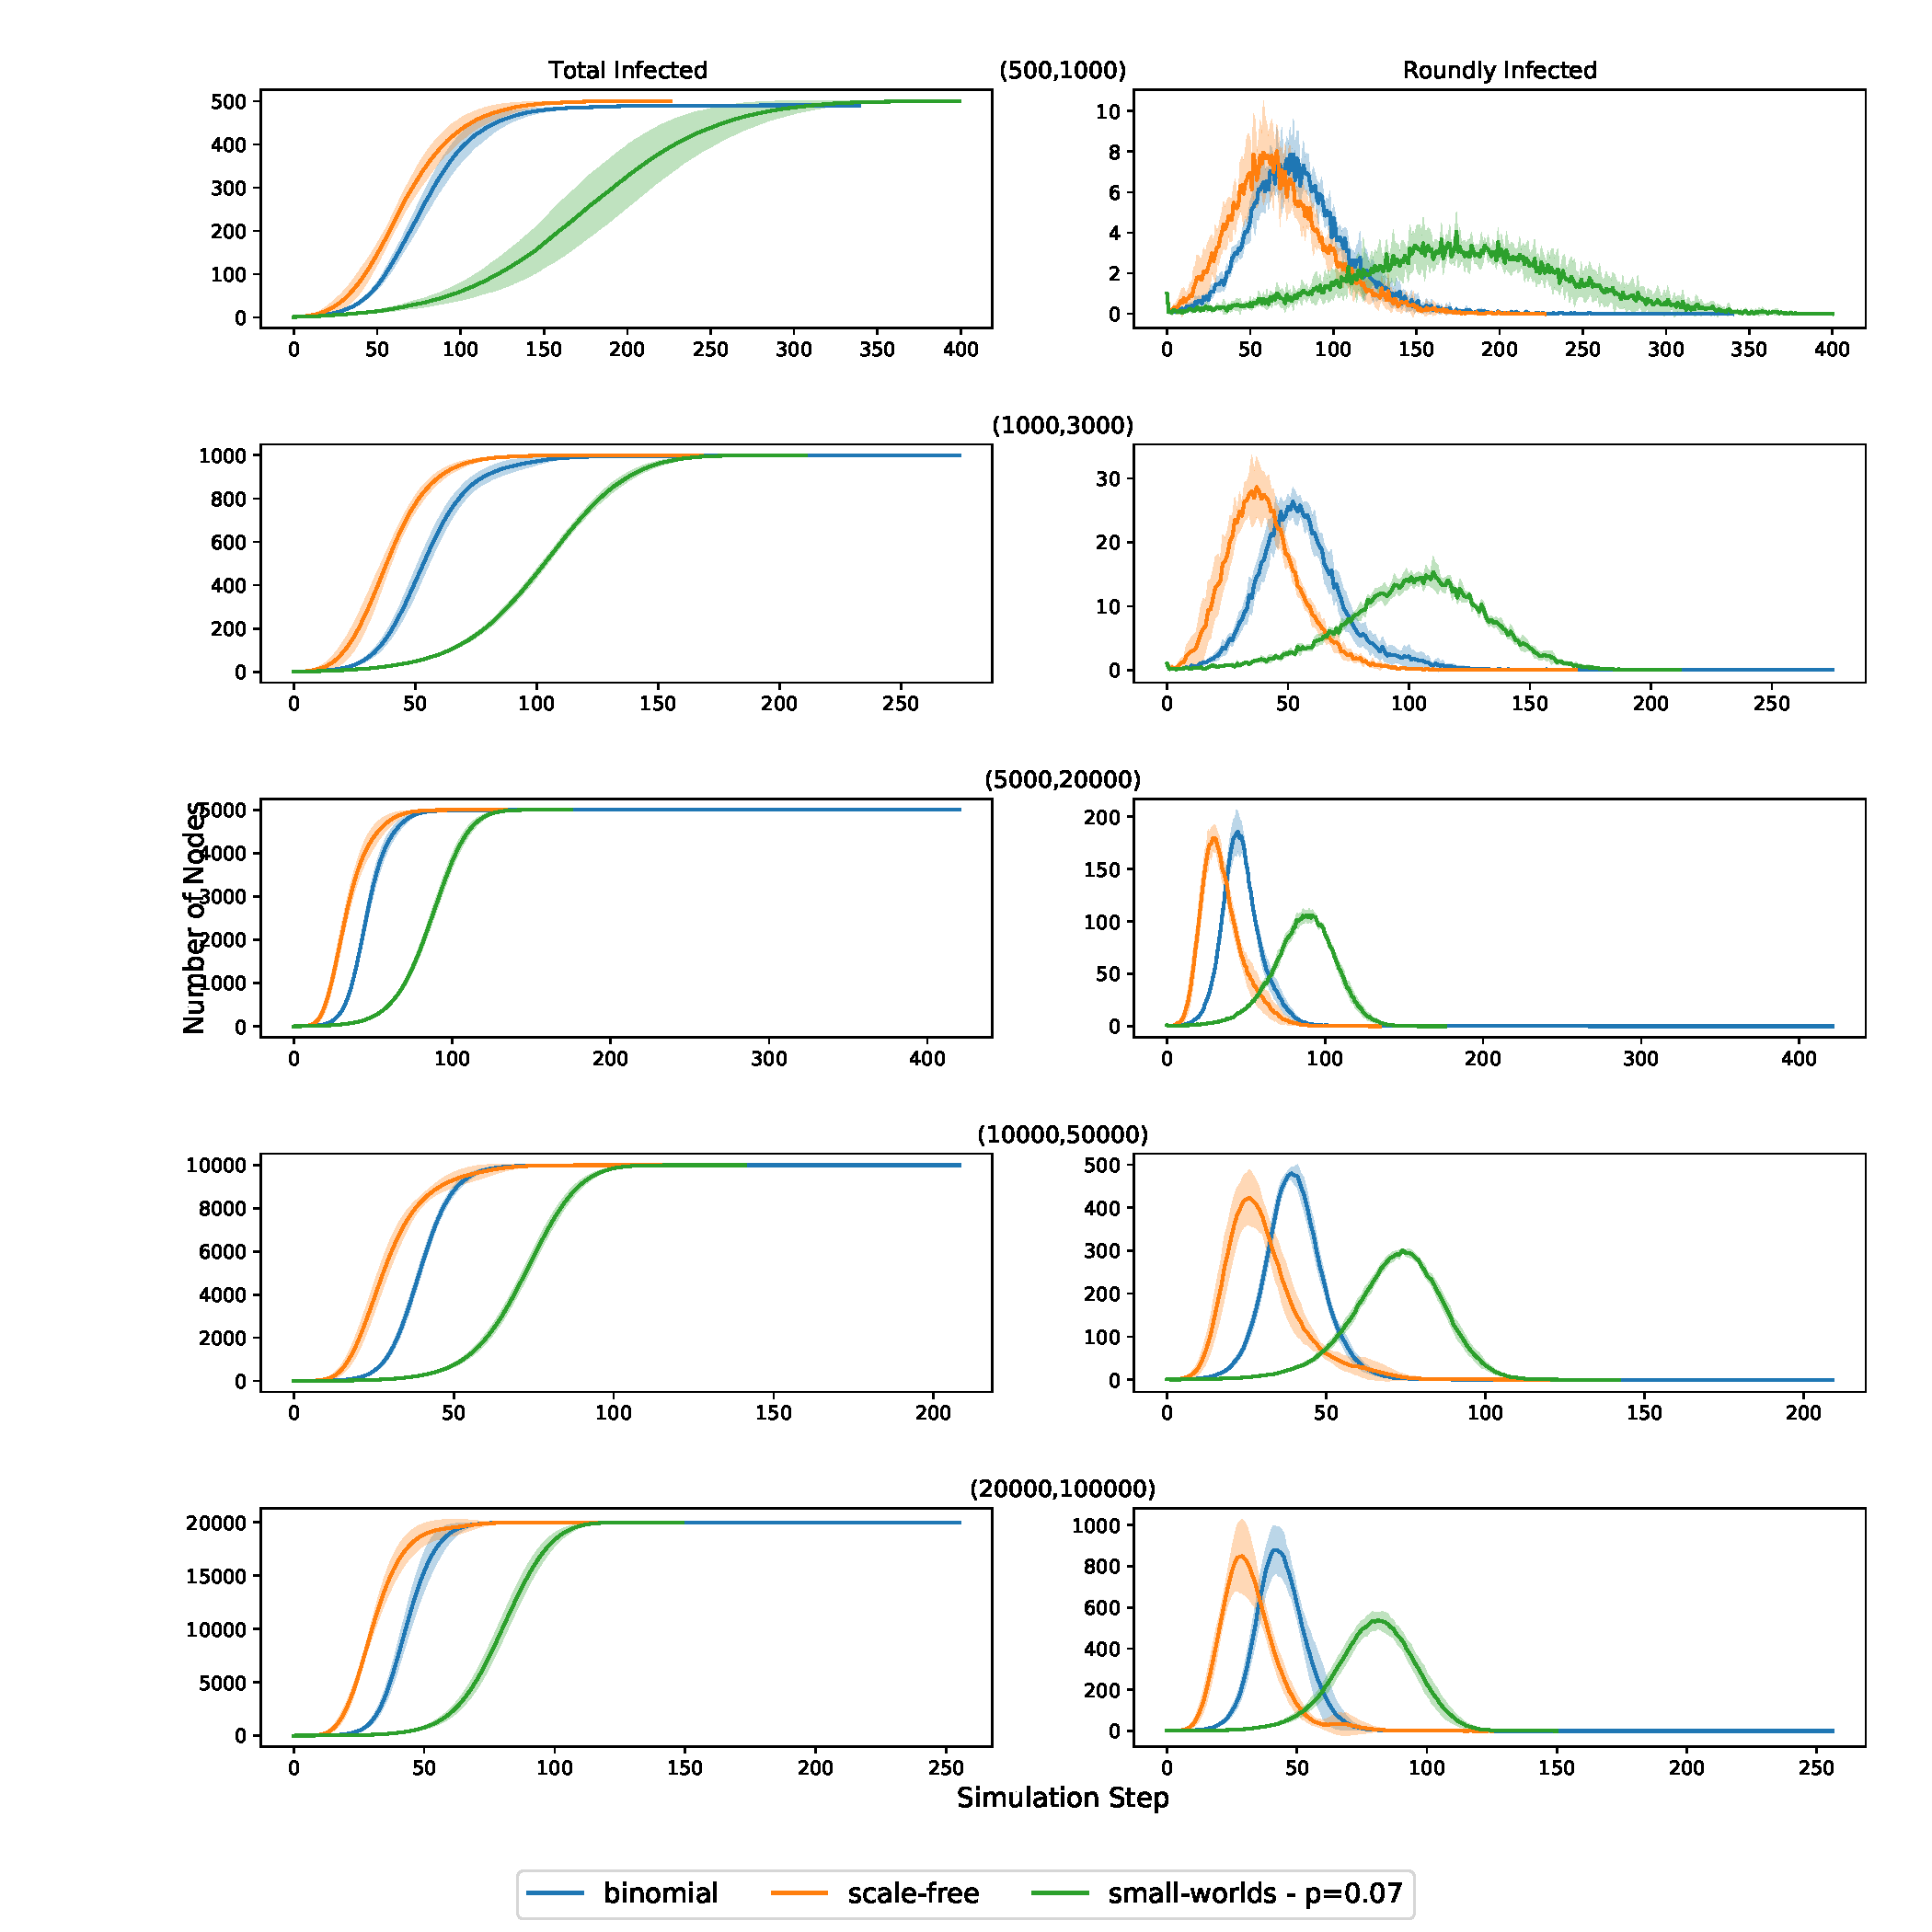
\includegraphics[width=0.5\textwidth]{img/pg1-sizes-compare_ms_p003.pdf}
  \end{center}
	\caption{Comparison of infection rates on graphs of different sizes. All figures use $p_{inf} = p_{cure} =  0.03$ and unlimited spread model.}
	\label{fig:pg2-sizes-compare_ms_p003}
\end{figure}

\begin{figure}[htb]
  \begin{center}
	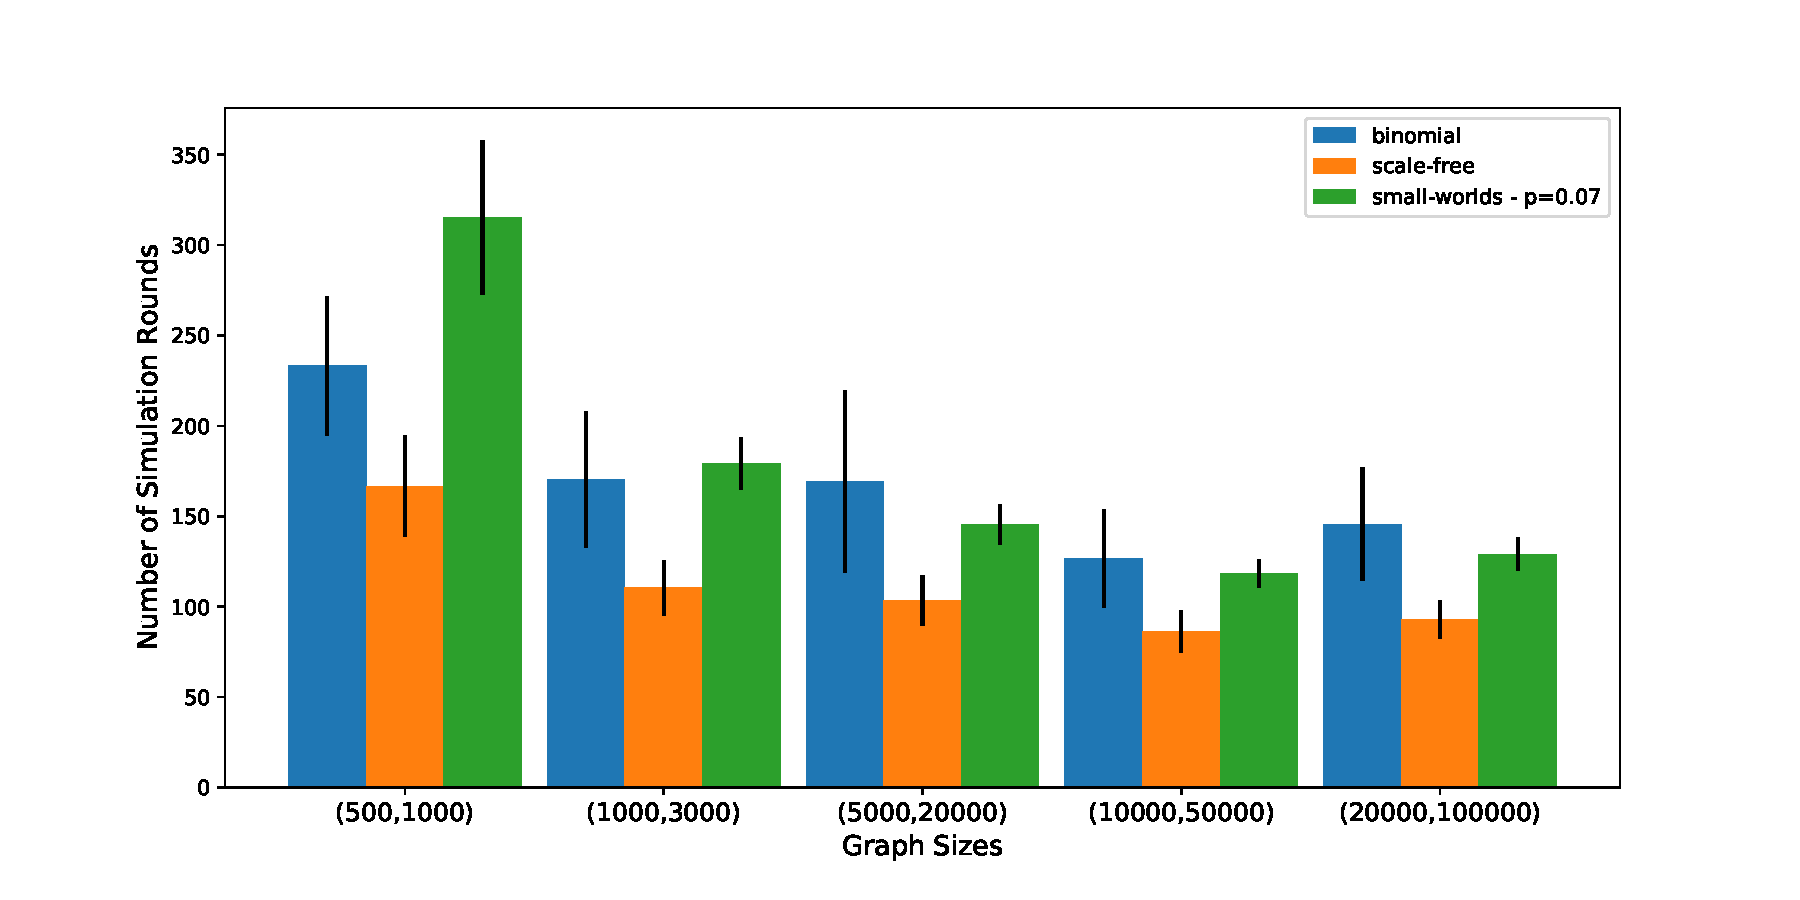
\includegraphics[width=0.5\textwidth]{img/pg1-sizes-compare_ms_003_bar.pdf}
  \end{center}
	\caption{Time to completely infect the network. All figures use $p_{inf} =  = p_{cure} = 0.03$ and unlimited spread model. Error bars show $\pm \sigma$.}
	\label{fig:pg2-sizes-compare_ms_003_bar}
\end{figure}

Figures \autoref{fig:pg2-sizes-compare_ms_p003} and \autoref{fig:pg2-sizes-compare_ms_003_bar} are provided for the sake of completeness, and don't directly add to the discussion.

\section{Discussions and Answers}\label{sec:disc-answers}

In this section, we will discuss the results to answer the questions.

\subsection{Question a)}\label{sec:question-a}

All of our experiments with program 1 show S-shape curve for total infection and bell-shape for roundly infection. This occurs because of the epidemic mechanics of a finite population. Initially, there are a few infected nodes, so they can only infect a small number of nodes every round. As the number of infected nodes increase, number of nodes they infect each round also increases. Since the number of infected nodes is still very small in comparison to whole population, it is safe to assume that most of their neighbors are still susceptible. Due to aforementioned observations, we see an exponential-like increase in roundly infections at the beginning.

However, at some point, number of infected nodes reaches to a point where most neighbors of infected nodes are also infected. Hence, the roundly infection numbers saturate. Then, finding susceptible nodes and infecting them gets increasingly difficult as only rather isolated nodes remain susceptible to this point. So, we see an exponential-like decrease in this part. As total number of infected nodes is just a running sum of this bell-shape; S-shape naturally follows. Intuitively, same arguments also hold for total infection too.

\subsubsection{Scale-free Networks}
Also, all of our results show that (eg. \autoref{fig:pg1-pis-compare_ms_5k}) the infection rate depends on the network topology. While the analysis done above hold for all; hence, we still see bell-shape and S-shape curves; the curves significantly and consistently differ between topologies.

Particularly in the unlimited infection resource scenario(see \autoref{sec:spread_model} for more information), infection spreads much faster in Scale-free networks. This is due to the fact that these networks are much more likely to have some hub nodes that are connected to many nodes. This speeds up the spread in two ways. Firstly, hubs are very likely to quickly get infected because as they have many neighbors; it is very likely that some of their neighbors are infected and gets them infected too. Then, infected hubs can very quickly spread the infection and they don't saturate for a long time, again thanks to having many neighbors.

Please see \autoref{sec:pg1-compare-pis} for an analysis of the spread model Prof. Ray proposed. It presents and discusses an interesting phenomenon of hubs becoming bottlenecks instead of super-spreaders.

\subsubsection{Small-worlds Networks}\label{sec:q1-small-worlds}

Moreover, we see that small-worlds networks having the slowest spread for the most part of the infection process. This is due to the fact that small-worlds graphs mostly look like a ring where each nodes are only connected to their closest neighbors. This in a way makes spreading a one-dimensional process; hence, greatly reduces the intersection between infected and susceptible nodes, ie. the infection can spread through only a few nodes.

But Watts-Strogatz networks also have a rewiring mechanism that creates shortcuts. These shortcuts create a possibility of jumps across the ring. These jumps allow the infection spread starting from different parts of the network. \autoref{fig:pg1-pis-compare_ms_5k}, indeed shows that increasing rewiring probability greatly speeds up the spread.


\subsubsection{Binomial Takes Longest to Fully Infect}\label{sec:binomial takes longest}

It is important to note that these analysis are made in terms of time to infect the "most" but not the "whole" of the network. When we look at the average time to infect the full network; binomial graphs take the longest.

This happens because in binomial graphs, it is likely to have some parts with very small connectivity and some parts with more connectivity. The parts with very small connectivity tends to be small too; so, most of the infection process is not affected from this. But, when we measure the time to fully infect the network; it can take a very long time to get these nodes infected.

On the other hand, while the arguments made in \autoref{sec:q1-small-worlds} still hold; all nodes in small-worlds networks initially have the same degree. This changes  with rewiring; but for small rewiring probabilities, it would be mostly maintained. Hence, there aren't such nodes with very small connectivity. This is also shown in \autoref{fig:pg1-pis-compare_ms_10k_bar}. Also, notice that error bars are much larger in binomial graphs. This is because they are the least structured random graphs among these three; hence, they exhibit more diverse behavior. In this case, some instances contain more small connectivity parts and some contain less; hence, leading to a wide spectrum of different infection times.

An exception is when the average degree is very small, as shown in \autoref{fig:pg1-sizes-compare_ms_003_bar}. Since the average degree is already too small in this case, the analysis of parts with very small connectivity doesn't effectively apply. For example, in $(500,1000)$ case, small-worlds nodes are only connected the nodes on their right and left; effectively creating a chain. This is already a thinly connected as possible, any less connectivity would create disconnected nodes.


\subsection{Question b)}

There are several similarities with the current pandemic. Firstly, \autoref{fig:pandemic} shows the daily and total cases, which is very similar to first half of the number of infected nodes curves that we obtained our experiments. This was expected as both are supposed be following a generic epidemic model.(See \cite{redcode}.)

\begin{figure}[htb]
  \begin{center}
	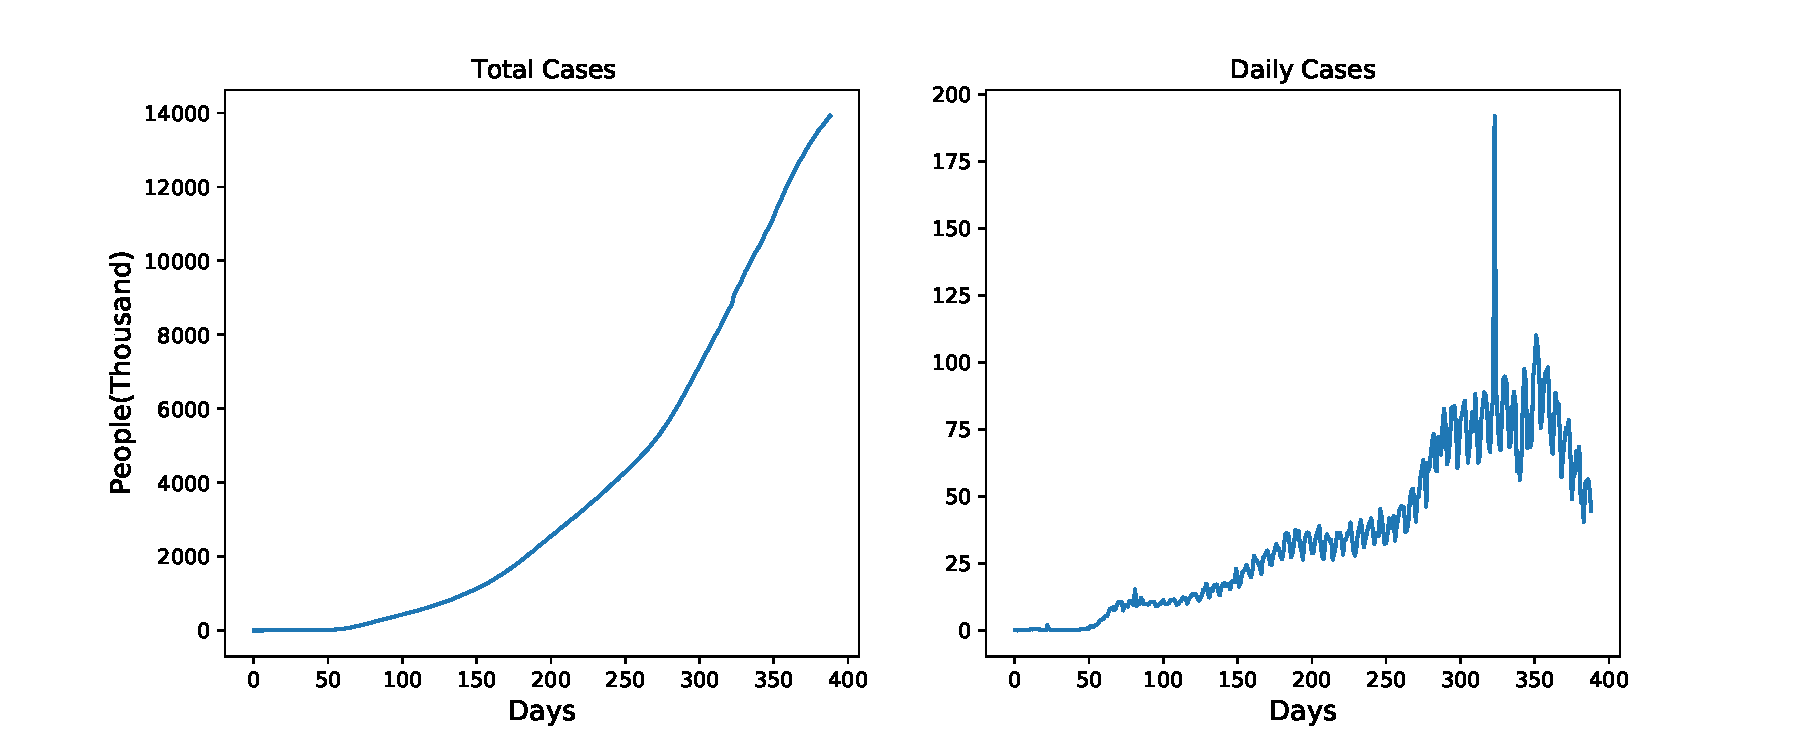
\includegraphics[width=0.5\textwidth]{img/pandemic.pdf}
  \end{center}
	\caption{Worldwide daily and total cases of COVID-19. Raw data is obtained from \url{https://ourworldindata.org/coronavirus-data and visualized}.}
	\label{fig:pandemic}
\end{figure}

Moreover, our results on how different topologies affect the spread give insights on how to reduce impacts of the pandemic.

For example, the fast spread in scale-free networks suggest that having active hubs in the society is problematic. These hubs can be markets, schools, workplaces. This is a loose comparison as these places are not actual nodes but groups of nodes with very high connectivity within and many connections to outside. However, the argument still holds that removing such places would help.

Also, the small spread in small-worlds networks in comparison to binomial networks is a supporting evidence for travel bans. Many critics, rightly, point out that no travel ban is perfect; and there are still people travelling between countries/cities, particularly between neighboring ones. But our results show that even such an imperfect travel ban is still quite useful. Those travelling people are accounted for in our model, through shortcuts of Watts-Strogatz and nodes being connected to their neighboring nodes. And still we see much smaller spread than binomial graphs.

\subsection{Question c)}

It reduces the infection rate. See \autoref{sec:pg2-res}, and in particular \autoref{sec:one2one-cure} for a detailed analysis.

\subsection{Question d)}

Without cure case was explained in detail in \autoref{sec:question-a}; so, we skip it to avoid being repetitive.

When a cure is used, as presented and discussed in \autoref{sec:pg2-compares-pis}, the infection can be cleaned from the networks with hub nodes faster. Particularly, see how binomial networks compare to small-worlds in with and without cure scenarios.

Moreover, networks with hub nodes exhibit a much higher variance. We believe that spread in this nodes highly depend on when hub nodes are cured. Again, see \autoref{sec:pg2-compares-pis} for future details.

\subsection{Question e)}

Building on our previous results and discussions, we believe that curing the nodes with highest degrees first would be a much better approach than random curing. This method should have the most impact in scale-free networks, which exhibits very high degree hub nodes. And it should be the least useful in small-worlds networks, as degrees of their nodes are very similar to each other.

To confirm our hypothesis, we generated 3 graph instances with (5000,20000) size from all three topologies and identified two nodes with highest degrees. Then, we run Program 2($p_{inf} = p_{cure} = 0.03$) on each graph twice: 1) initially curing random 2 nodes 2) initially curing the identified hub nodes.\autoref{fig:smartcure-randomcure} shows that our approach leads to significant benefits. Also, our analysis on how each topology will be affected was accurate.

\begin{figure}[htb]
  \begin{center}
	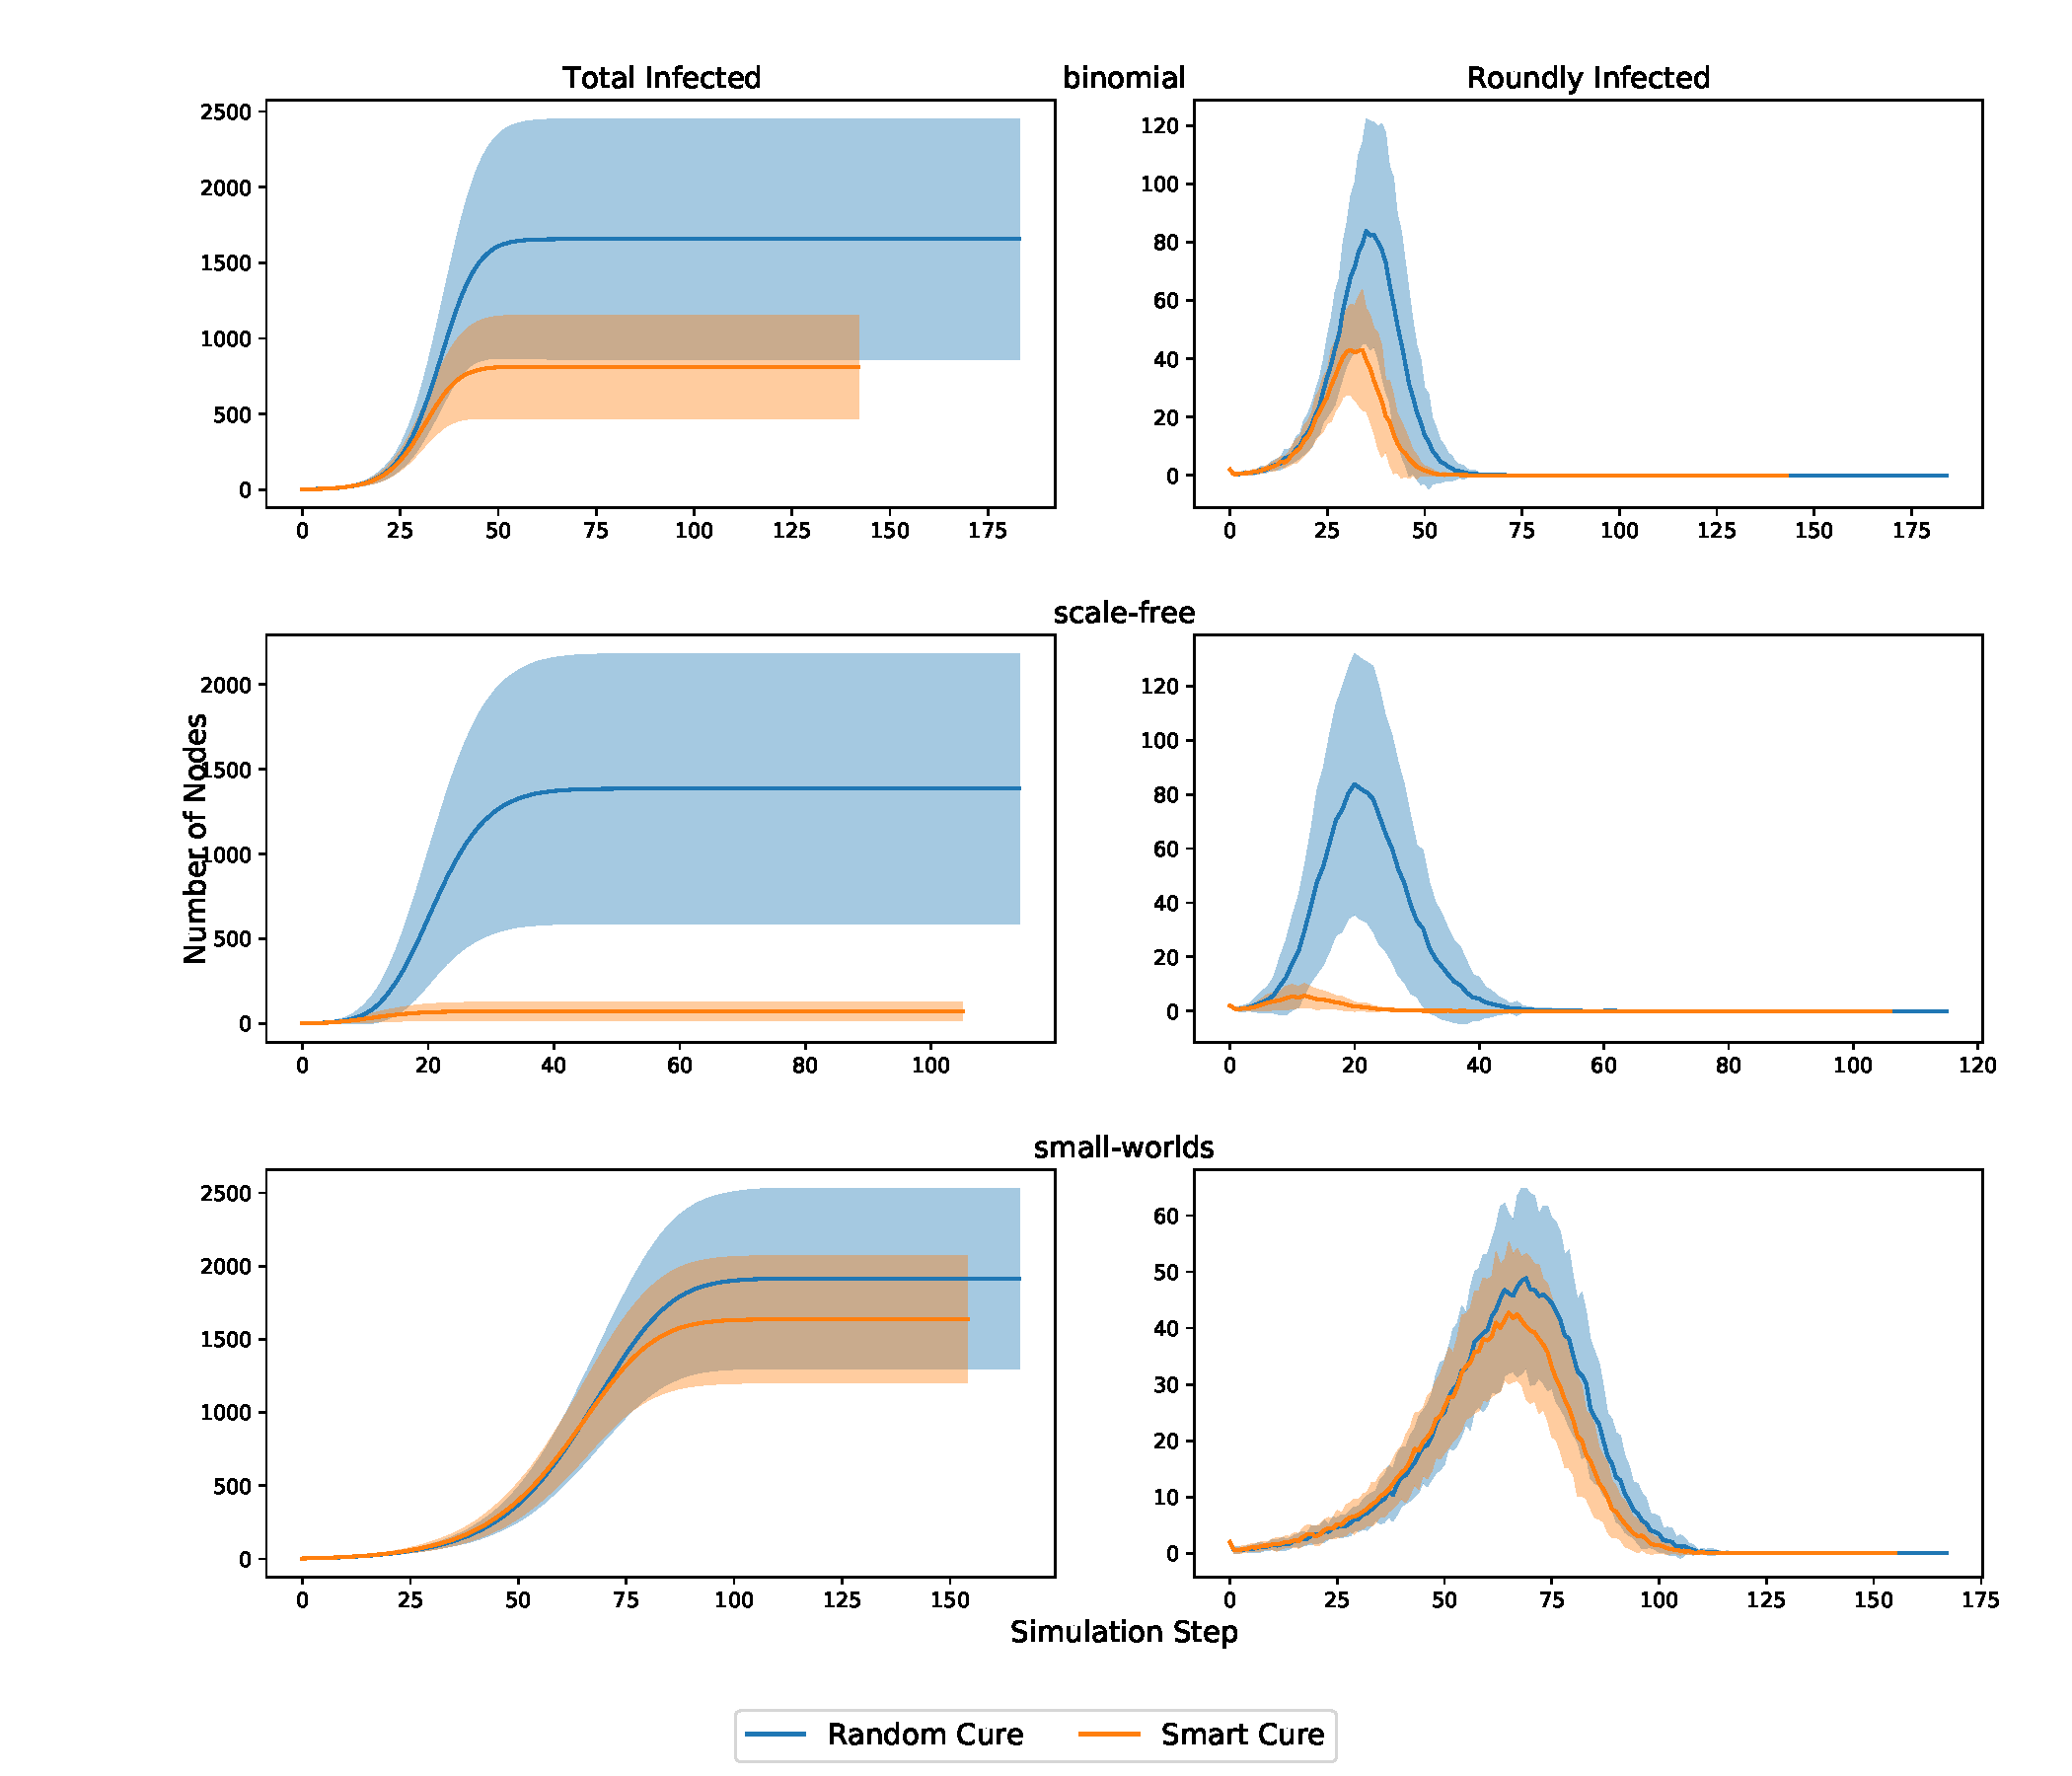
\includegraphics[width=0.5\textwidth]{img/smartcure-randomcure.pdf}
  \end{center}
	\caption{Infection spread comparison between random initial curing and "smart" initial curing.}
	\label{fig:smartcure-randomcure}
\end{figure}


\section{Conclusion}

In this work, we've investigated worm propagation in topology constrained networks both with and without a cure. Our results show that topology of the networks has a great impact in infection spread behaviors.

Finally, in \autoref{sec:disc-answers}, answer and discuss the questions in project proposal. Source code for this work can be found on \url{www.github.com/alperentercan/worm-propagation}.



% \FloatBarrier{}
\bibliographystyle{IEEEtran}
\bibliography{topology_constrained_redcode}

\end{document}
